% указываем класс документа
\documentclass[12pt,a4paper,openany]{extarticle}
% подключаем собственный стилевой файл 
\usepackage{mystyle}
% указываем язык (для автоматической вставки слов, типа "Глава", "Содержание", "Литература", "рис." и пр.
\selectlanguage{russian}
\graphicspath{{./images/}}
\usepackage[pdftex]{lscape}

\begin{document}

\part*{Лабораторная работа №4\\
Настройка ПИД-регулятора}

\section{Методические рекомендации}
\hspace*{\parindent}До начала работы студент должен выполнить предыдущие лабораторные этого цикла.

\section{Теоретические сведения}
\hspace*{\parindent}В~прошлой лабораторной работе было необходимо повернуть выходной вал мотора EV3 на  определенный угол.
Путем применения П-регулятора эта цель по большому счету достигалась, и вал оказывался вблизи требуемого положения. 
При этом можно было заметить, что указанный процесс характеризовался среди прочего, во-первых, отличной от нуля установившейся ошибкой управления, выражающейся в недовороте или перелете вала на несколько градусов относительно желаемого положения, а во-вторых, появлением перерегулирования при увеличении значения коэффициента регулятора. 
Данные особенности могут быть нежелательными или даже неразрешенными при решении реальных практических задач, а поэтому в таких ситуациях необходимо использовать иные приемы управления, которые либо совсем свободны от указанных явлений, либо подвержены им в меньшей степени. Одной из таких стратегий управления является ПИД-регулятор.
Рассмотрение его сути предварим рассмотрением более простых П-, И- и Д-регуляторов.

\paragraph*{ПИД-регулятор}$\phantom{-}$\\
\hspace*{\parindent}П-регулятор, как стало известно из прошлой лабораторной, предполагает подачу в систему в качестве управляющего воздействия ($U$) результата произведения некоторого постоянного коэффициента ($k_P$) на разность желаемого значения регулируемой величины ($y_w$) и ее текущего значения ($y$), то есть описывается выражением:
\begin{equation}
U = k_P(y_w - y) = k_P e\ldotp
\end{equation}
Интегральный регулятор (И-регулятор) определяет сигнал управления как интеграл от ошибки~$e$, умноженный на некоторый постоянный коэффициент $k_I$:
\begin{equation}
U = k_I\int\limits_{t_0}^{t_1} \!e\,dt,
\end{equation} 
дифференциальный регулятор (Д-регулятор)~--- как производную по времени от $e$, умноженную на постоянный коэффициент $k_D$:
\begin{equation}\label{eq:definiton_of_D_regulator}
U = k_D\dot{e}\ldotp
\end{equation}

Как правило, в качестве самостоятельных регуляторов И- и Д-регуляторы не применяются.
Собственно, это объяснимо.

Дело в том, что если попытаться достичь нужного значения изменяемой величины применением только Д-регулятора, ничего в итоге не получится.
\underline{Лучшее}, что c его помощью можно достигнуть~--- это сравнять производную выходной величины $y(t)$ системы с производной функции $y_w(t)$, описывающей желаемое изменение во времени величины $y$.
Почему так происходит, можно понять после более внимательного рассмотрения формулы~\eqref{eq:definiton_of_D_regulator}.
Конкретно должно броситься в глаза то, что она совпадает по строению с уравнением такого П-регулятора, который бы мы применили, если бы хотели добиться указанного выше эффекта:
\begin{equation}
U = k_D\dot{e} = k_D(\dot{y_w} - \dot{y})\ldotp
\end{equation}
Описанная особенность хорошо демонстрируется результатами моделирования схем, показанных на рис.~\ref{fig:D_regulator} и~\ref{fig:D_regulator_linear_g}.
Как можно видеть из их строения, они описывают процессы управления углом поворота ротора двигателя постоянного тока с помощью Д-регулятора.
В полном согласии со сказанным ранее не при $\theta_w(t)=50^\circ=const$ и, следовательно, $\dot{\theta}_w(t) = 0$, что справедливо для схемы с рис.~\ref{fig:D_regulator}, не при $\theta_w(t) = 50^\circ t$ и, следовательно, $\dot{\theta}_w = 50^\circ$ (справедливо для схемы с рис.~\ref{fig:D_regulator_linear_g}) равенство $\theta(t)=\theta_w(t)$ Д-регулятор не обеспечивает (см.~рис.~\ref{fig:D_regul_const_g} и~\ref{fig:D_regul_linear_g_graphs}).
Лучший результат, которого он добивается в описанных случаях~--- это поддержание равенства $\dot\theta(t)=\dot\theta_w(t)$ при $\theta_w(t)=50^\circ=const$ (см.~рис.~\ref{fig:D_regul_const_g}).

\begin{figure}[h!]
	\centering{ 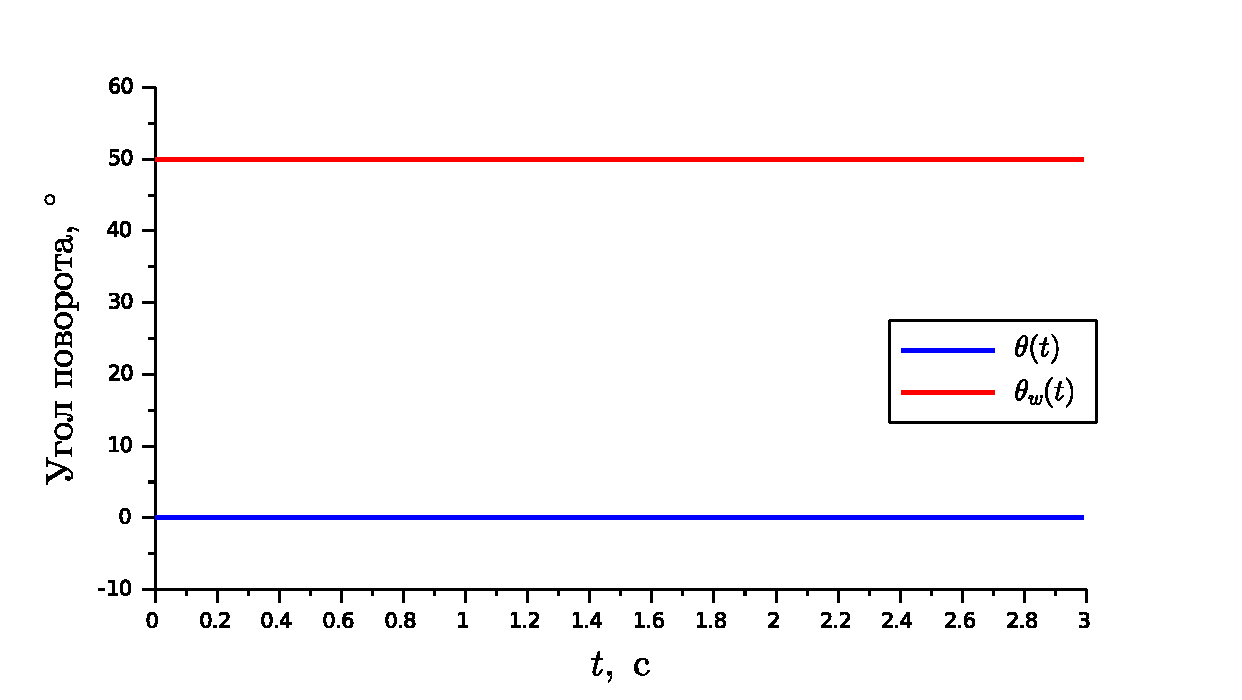
\includegraphics[width = 15cm]{D_regul_const_g.pdf} }
	\vspace{-0.5cm}
	\caption{Графики, демонстрирующие отработку Д-регулятором сигнала задания $\theta_w(t) = 50^\circ$.}
	\label{fig:D_regul_const_g}
\end{figure}	
	
\begin{landscape}
\thispagestyle{empty}
\begin{figure}[h!]
	\centering{ 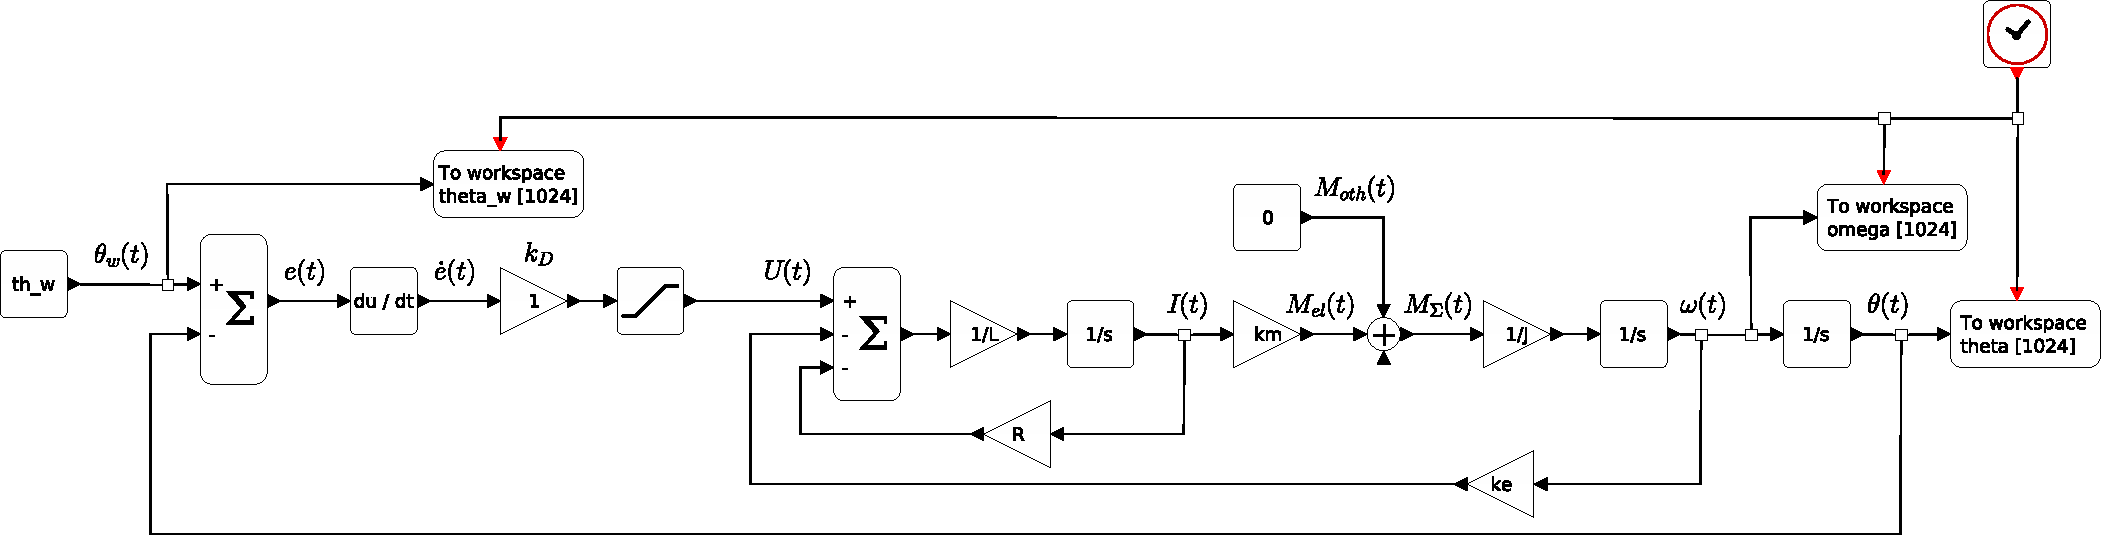
\includegraphics[width = 25cm]{D_regulator.pdf} }
	\caption{Схема моделирования процесса управления двигателем постоянного тока с помощью Д-регулятора при $\theta_w(t) = const$.}
	\label{fig:D_regulator}
\end{figure}	

\begin{figure}[h!]
	\centering{ 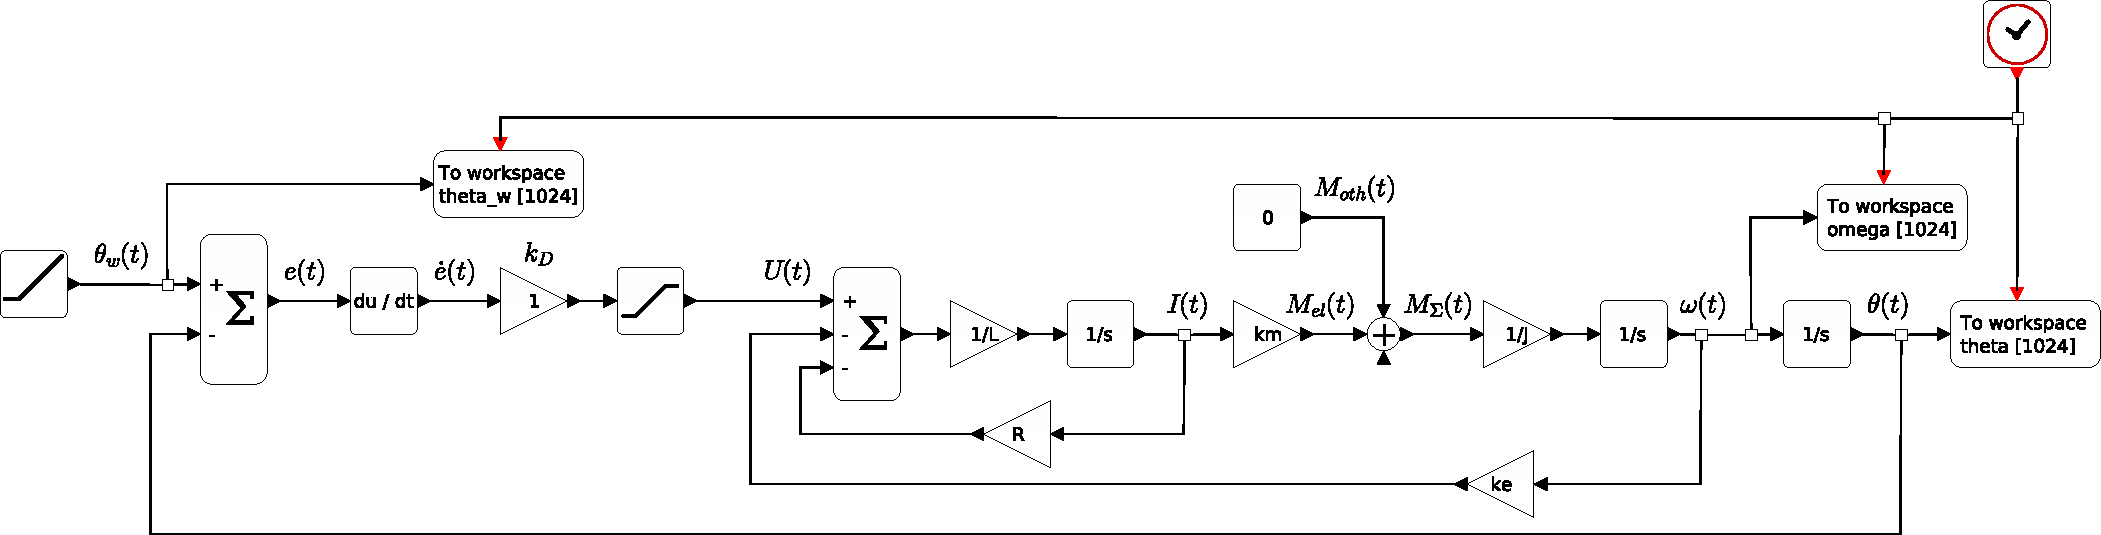
\includegraphics[width = 25cm]{D_regulator_linear_g.pdf} }
	\caption{Схема моделирования процесса управления двигателем постоянного тока с помощью Д-регулятора при $\theta_w(t) = 50^\circ t$.}
	\label{fig:D_regulator_linear_g}
\end{figure}	

\end{landscape}

\begin{figure}[h!]
	\centering{ 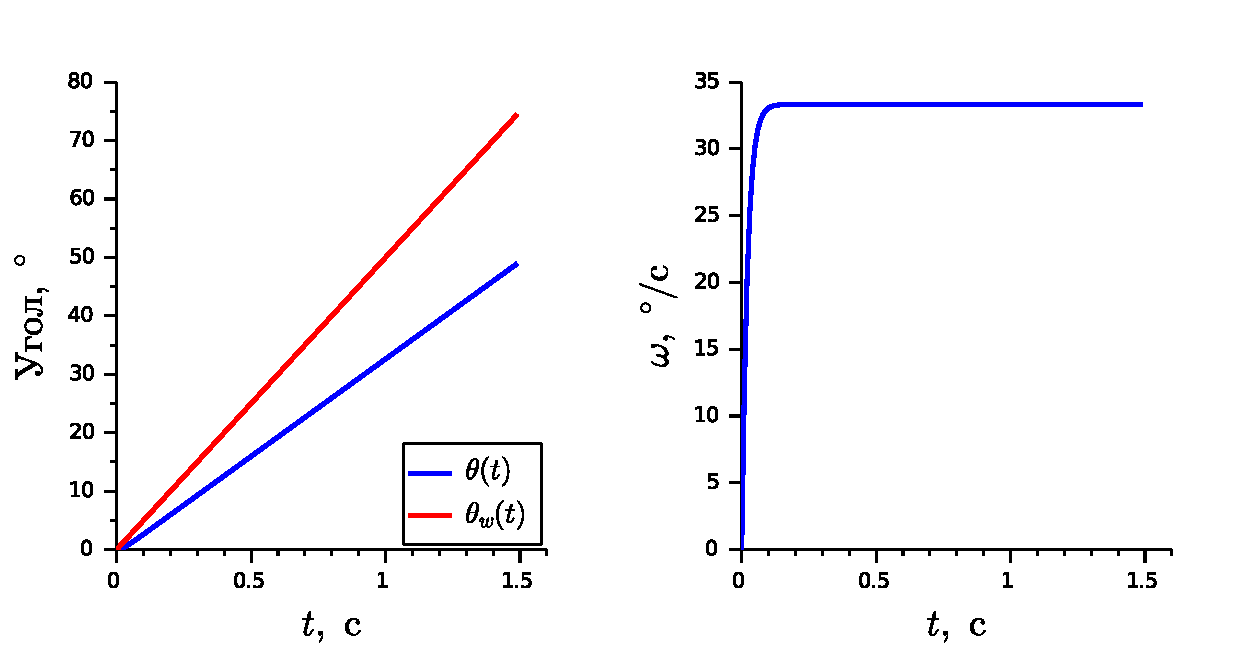
\includegraphics[width = \textwidth]{D_regulator_linear_g_graphs.pdf} }
	\vspace{-1cm}
	\caption{Графики, демонстрирующие отработку Д-регулятором сигнала задания $\theta_w(t) = 50^\circ t$.}
	\label{fig:D_regul_linear_g_graphs}
\end{figure}

Система, предоставленная управлению одного И-регулятора, также далека от надежной.
Несмотря на то, что могут быть случаи, в которых И-регулятор справится со своей задачей и по некотором времени обеспечит выполнение равенства $y = y_w$, в остальных ситуациях он приведет к тому, что значение величины $y$ начнет с постоянной или даже со все более возрастающей амплитудой колебаться около желаемого значения $y_w$.

Чтобы понять, почему произойдет именно так, достаточно представить себе процесс работы И-регулятора.
Предположим, что в нашем распоряжении есть система, выходная величина которой находится на уровне $y = y_0 < y_w$.
Далее мы, грубо говоря, включаем И-регулятор.
В~начальный момент времени интеграл от ошибки $y_w - y$ равен нулю, и, следовательно, на систему не будет подано никакого управляющего воздействия.
В~дальнейшие моменты времени значение интеграла ошибки будет расти.
Вместе с ним будет расти и управляющее воздействие, подаваемое на систему.
Под действием последнего система начнет движение, при котором величина $y$ будет приближаться к значению $y_w$.
Поскольку весь этот процесс будет характеризоваться положительным значением ошибки, то интеграл от нее будет продолжать расти, пусть уже и медленнее.
Спустя некоторое время система придет в состояние $y = y_w$, но, так как интеграл от ошибки, а значит и управляющее воздействие, при этом никак не изменится, система не остановится в этом положении, а продолжит свое движение в сторону значений $y$, превышающих $y_w$.
Значения ошибок регулирования при этом станут отрицательными.
Следовательно начнет уменьшаться накопленный интеграл ошибки.
Спустя некоторое время, в течение которого система будет продолжать свое движение, интеграл уменьшится до нуля.
В~этот момент времени управляющее воздействие также упадет до нуля и величина $y$ перестанет изменяться.
В~дальнейшем из-за непрекращающегося уменьшения интеграла его значение станет отрицательным, а значит $y$ начнет свое движение в направлении, противоположном тому, в котором он двигался до этого.
После этого с тем отличием, что значение $y$ будет изменяться в другую сторону, весь процесс начнет повторяться.
Собственно, описанные колебания системы и могут быть незатухающими.

Так, к примеру, происходит с углом поворота ротора двигателя постоянного тока.
Это можно наблюдать на рис.~\ref{fig:I_regul_const_g}, на котором показаны графики зависимостей $\theta(t)$ и $U(t)$, построенные по данным, полученным в результате моделирования схемы, показанной на рис.~\ref{fig:I_regul_scheme}.

\begin{figure}[h!]
	\centering{ 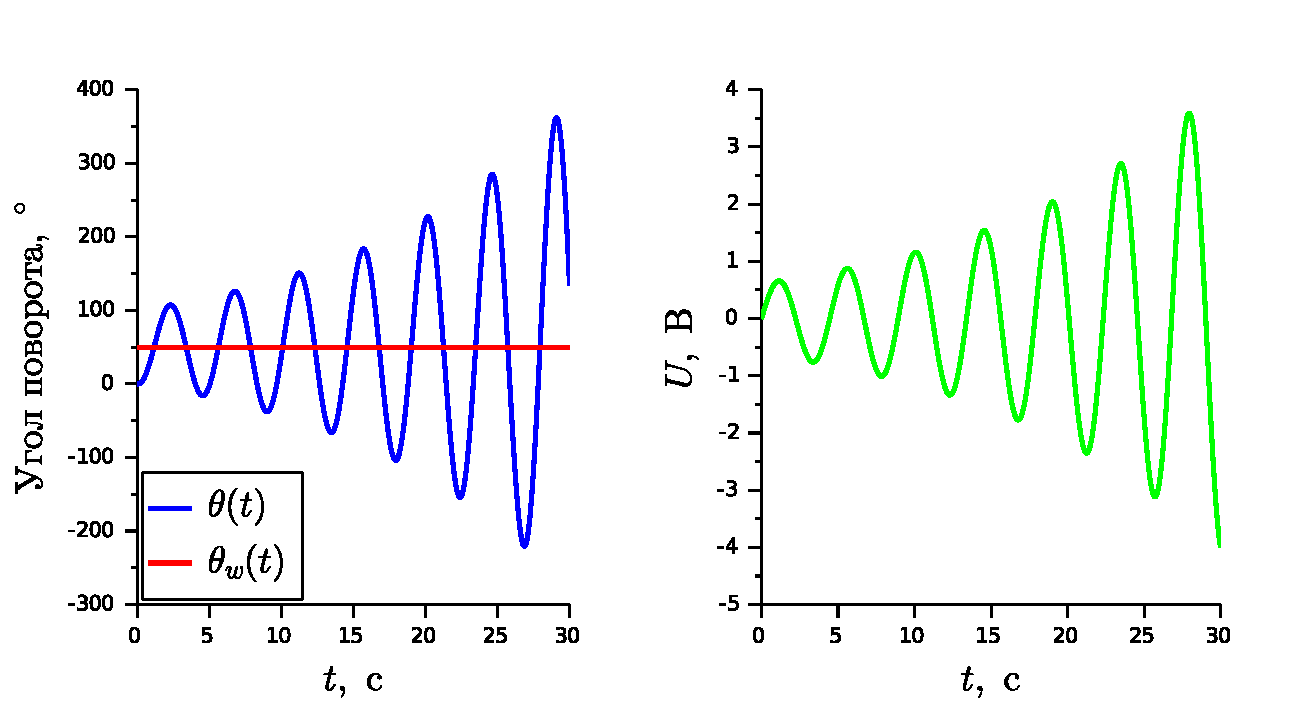
\includegraphics[width = \textwidth]{I_regul_const_g.pdf} }
	\vspace{-1cm}
	\caption{Графики, демонстрирующие отработку И-регулятором сигнала задания $\theta_w(t) = 50^\circ$.}
	\label{fig:I_regul_const_g}
\end{figure}

Обычно И- и Д-регуляторы объединяются с П-регулятором в более сложные регуляторы, такие как ПИ-, ПД- и ПИД-регулятор.
Под <<объединяются>> следует понимать тот факт, что, например, управляющее воздействие, формируемое ПИ-регулятором, есть сумма управляющих воздействий его П- и И-составляющих:
\begin{equation}
U = k_Pe + k_I\int\limits_{t_0}^{t_1} \!e\,dt,
\end{equation}
а управляющее воздействие на выходе ПИД-регулятора есть сумма управляющих воздействий, создаваемых П-, И- и Д-регуляторами, входящими в его состав:
\begin{equation}
U = k_Pe + k_I\int\limits_{t_0}^{t_1} \!e\,dt + k_D\dot{e}\ldotp
\end{equation}
При таких объединениях И- и Д-составляющие начинают выполнять полезные функции. Рассмотрим их.

Введение в управляющее воздействие Д-регулятора приводит к уменьшению колебаний системы.
Этот эффект несложно объясним.
При отклонении системы от нужного положения скорость изменения регулируемой величины совпадает по знаку с самим отклонением, а значит Д-составляющая помогает П-регулятору препятствовать указанному отклонению.
После же того, как регулируемая величина закончит изменяться в первоначальном направлении и начнет изменяться в другом, знак составляющей управляющего воздействия, формируемой дифференциальным регулятором, станет противоположным знаку управляющего сигнала пропорционального регулятора.
Значит Д-регулятор будет препятствовать возвращению П-составляющей регулируемой величины в нужное состояние.
Таким образом дифференциальная составляющая будет в некоторой степени притормаживать движение системы в сторону желаемого значения и тем самым препятствовать перелету регулируемой величины через требуемое значение, которое может происходить при применении только П-регулятора.

Описанную особенность можно наблюдать в графиках (см.~рис.~\ref{fig:PD_regul_advantages}), демонстрирующих результат моделирования схемы, представленной на рис.~\ref{fig:PID_regul_scheme} при $M_{oth}=0\text{ Н}{\cdot}\text{м}$, $\theta_w(t) = \pi/2$, $k_I = 0\text{ В}/(\text{рад}{\cdot}\text{с})$ и $k_P = 20\text{ В/рад}$.
Как видно из указанного рисунка, применение ПД-регулятора и вправду снижает колебательность переходных процессов. 

\begin{figure}[h!]
	\centering{ 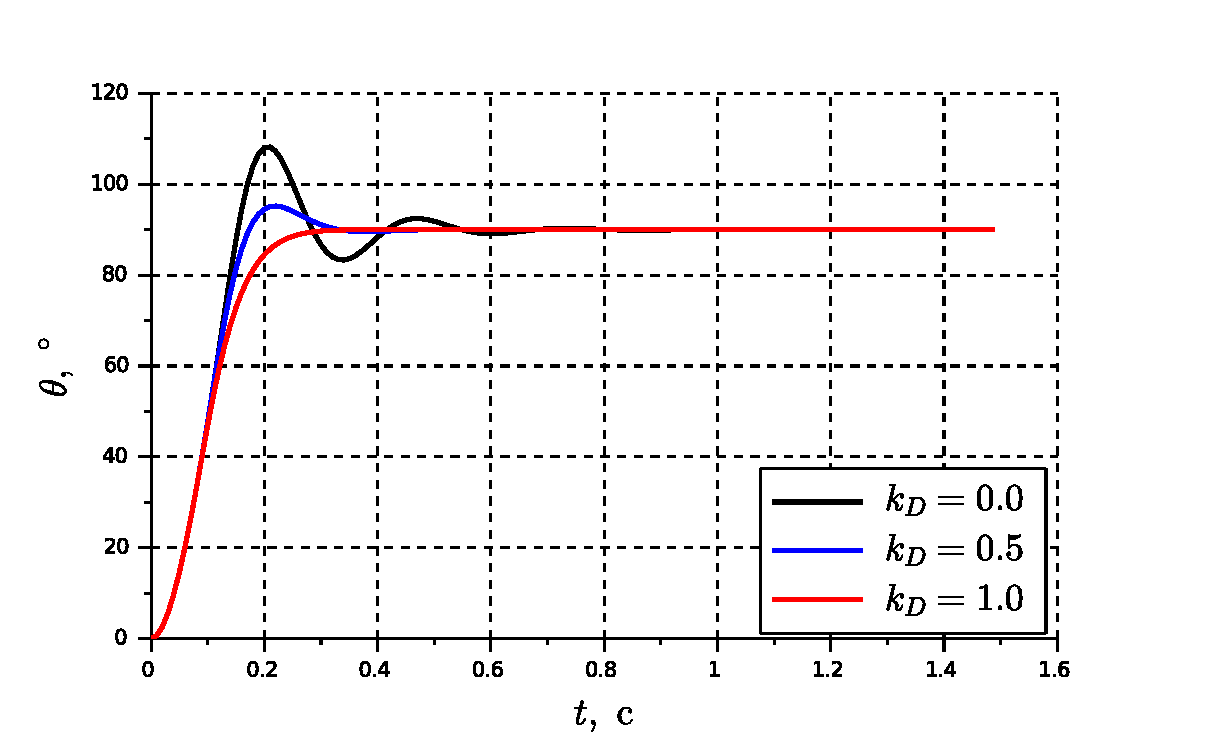
\includegraphics[width = 0.9\textwidth]{PD_regul_advantages.pdf} }
	\vspace{-0.5cm}
	\caption{Графики, демонстрирующие пользу от добавления Д-составляющей.}
	\label{fig:PD_regul_advantages}
\end{figure}	

Дополнительно про дифференциальную составляющую можно отметить, что из-за нее может повышаться быстродействие системы (все-таки быстрее затухающим колебаниям соответствует меньшее время переходного процесса), однако, если значение коэффициента $k_D$ сделать слишком большим, то можно наткнуться на противоположный эффект: быстродействие системы начнет снижаться.
Последнее будет происходить по той причине, что в этом случае Д-составляющая будет уже больше мешать П-регулятору, чем полезно дополнять его, и тормозить движения системы.

Использование в управлении И-регулятора помогает убирать установившееся значение ошибки регулирования.
Сказанное хорошо демонстрируется на примере задачи из прошлой работы.
Как можно из нее помнить, П-регулятор (особенно при небольших коэффициентах) при нахождении вала вблизи желаемого положения не мог сформировать управляющего напряжения, которое бы обеспечило мотору момент силы, превосходящий действующие на его подвижную часть силы сопротивления, и, следовательно, вал мотора не доворачивался до нужного положения.
Если бы для этой задачи использовался ПИ-регулятор, такой проблемы не было бы.
Объяснить это не сложно.
Предположим, что вал мотора EV3, находящегося под управлением ПИ-регулятора, остановился в нескольких градусах от требуемого положения. Довернуться в него мешают действующие на него силы сопротивления (силы трения, моменты нагрузки и т. д.).
В описанной ситуации система будет характеризоваться отличным от нуля значением ошибки.
Значит, интегральная часть будет расти.
Значит, спустя некоторое время формируемый ею сигнал управления достигнет такого значения, при котором вызываемый им крутящий момент $M_{el}$ вырастет так, что превысит выше упомянутые силы сопротивления.
Значит, двигатель все-таки довернется в нужное положение.

Показательным примером сказанному могут быть графики, представленные на рис.~\ref{fig:PI_regul_achievs}.
Они являют собой результат моделирования схемы, продемонстрированной на рис.~\ref{fig:PID_regul_scheme}, при $M_{oth} = -0.2\text{ Н}{\cdot}\text{м}$, $\theta_w(t)=\pi$, $k_D = 0\text{ В}{\cdot}\text{с}/\text{рад}$ и $k_P = 15\text{ В/рад}$.
Характер этих графиков подтверждает ранее озвученное преимущество, даваемое И-регулятором: на зеленом графике ошибка управления стремится к нулю.

\begin{figure}[h!]
	\centering{ 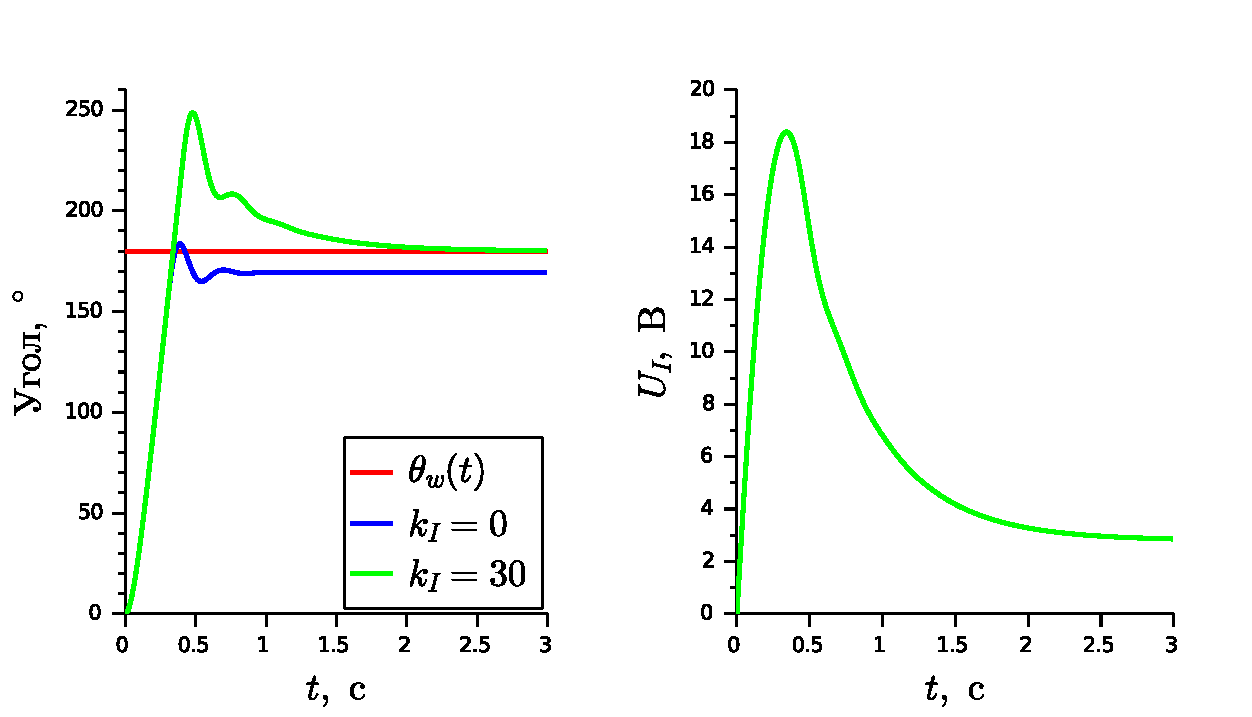
\includegraphics[width=\textwidth]{PI_regul_achievs.pdf} }
	\vspace{-1cm}
	\caption{Графики, демонстрирующие пользу от добавления интегральной составляющей.}
	\label{fig:PI_regul_achievs}
\end{figure}	


\begin{landscape}
\thispagestyle{empty}
\begin{figure}[h!]
	\centering{ 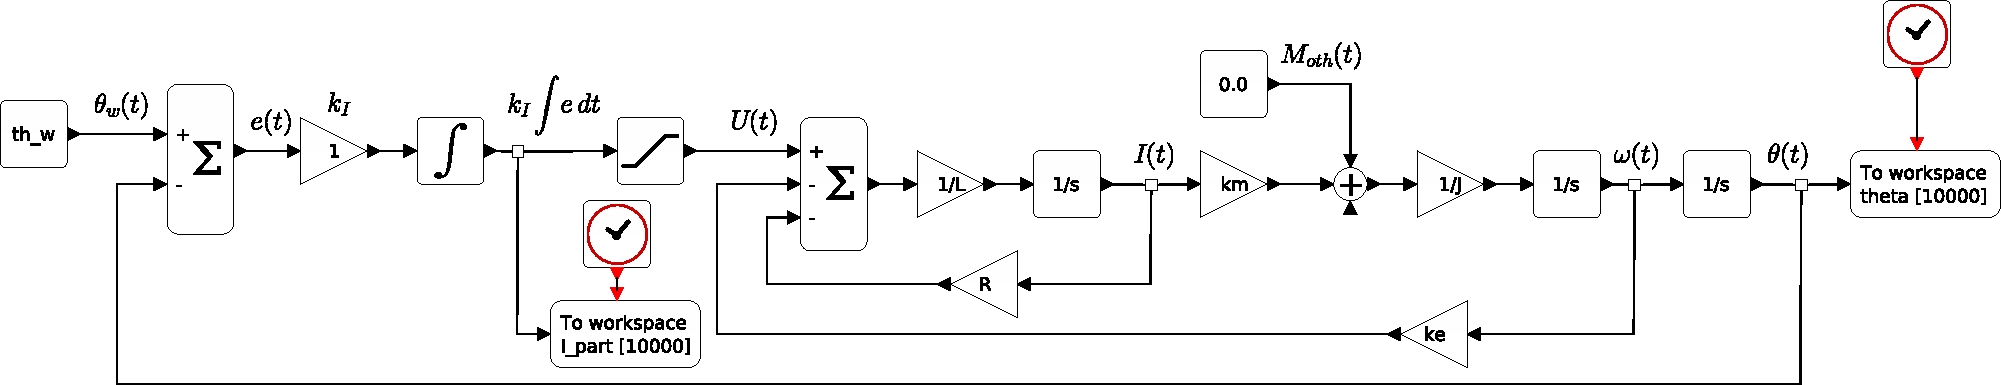
\includegraphics[width = 27cm]{I_regul_scheme.pdf} }
	\caption{Схема моделирования процесса управления двигателем постоянного тока с помощью И-регулятора при $\theta_w(t) = const$.}
	\label{fig:I_regul_scheme}
\end{figure}	

\begin{figure}[h!]
	\centering{ 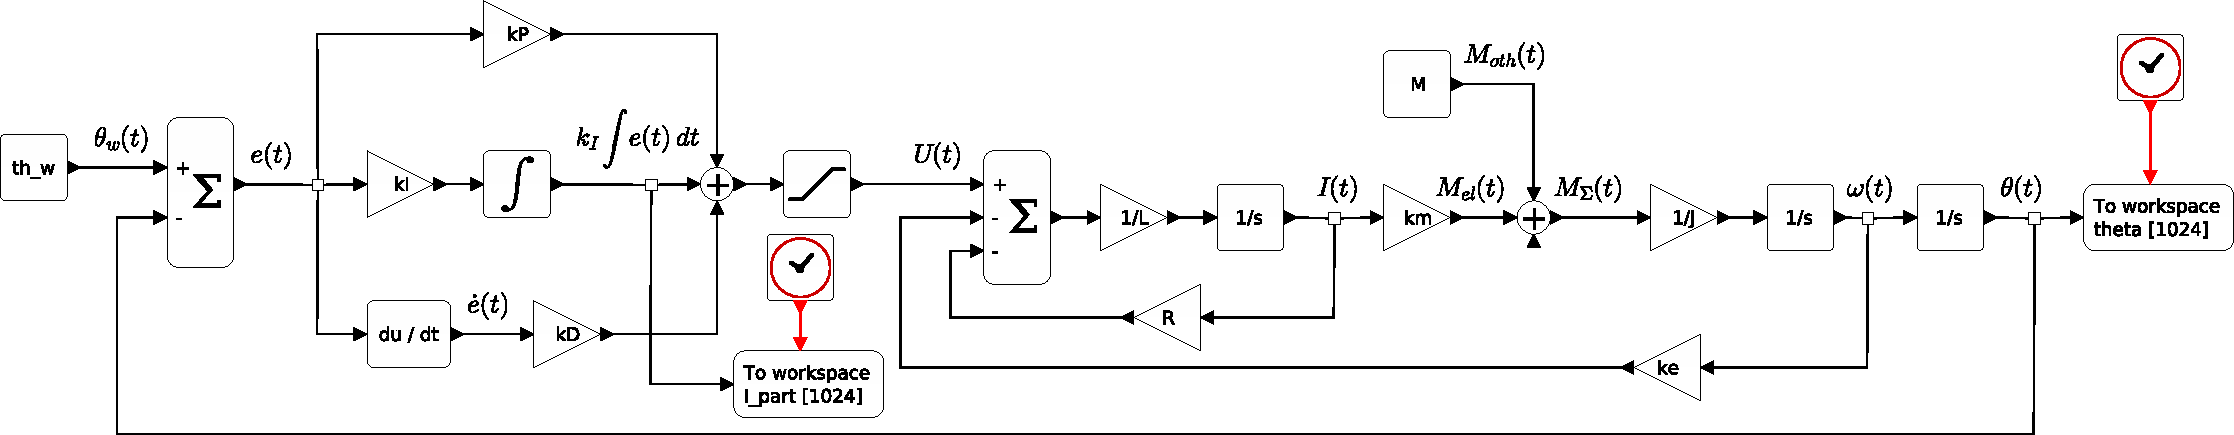
\includegraphics[width = 27cm]{PID_regul_scheme.pdf} }
	\caption{Схема моделирования процесса управления двигателем постоянного тока с помощью ПИД-регулятора при $\theta_w(t) = const$.}
	\label{fig:PID_regul_scheme}
\end{figure}	

\end{landscape}

Последние графики, относящиеся к работе системы управления с ПИ-регулятором, помимо всего прочего показывают, что для изменения управляющего воздействия $U_I$, формируемого интегральной составляющей, необходимо значительное время.
Поскольку указанная особенность ухудшает качество переходных процессов, для борьбы с ней применяют схемы (приемы), ограничивающие рост значения $U_I$.
Такие схемы, или приемы, называются схемами (приемами) anti-windup, или просто anti-windup.
И, надо сказать, применение приемов anti-windup приводит к улучшению динамики систем.

На рис.~\ref{fig:anti_windup_schemes} показана схема моделирования процессов работы двух простых приемов anti-windup: <<обрезки>> текущего значения интеграла ($a$) до определенного уровня ($b$) и ограничения роста его значения этим же уровнем\footnote{Такое ограничение включается и регулируется параметрами внутренней настройки блока с изображением интеграла, которые оказываются доступными для редактирования после, например, выделения блока и нажатия клавиш Ctrl+B.} ($c$).
Графики, поясняющие их работу, приведены на рис.~\ref{fig:anti_windup_graphs}.
Как можно видеть, в обеих схемах значение интеграла ограничивалось уровнем, равным~$8$.

Применение второй из указанных схем anti-windup ($c$) при уровне ограничения управления $U_I$, равном~$4\text{ В}$, к рассмотренному ранее ПИ-регулятору ($k_P = 15$, $k_I = 30$) и той же системе моделирования приводит к улучшению качества переходных процессов так, как это показано на рис.~\ref{fig:PI_regul_with_anti_windup}.

\begin{figure}[h!]
	\centering{ 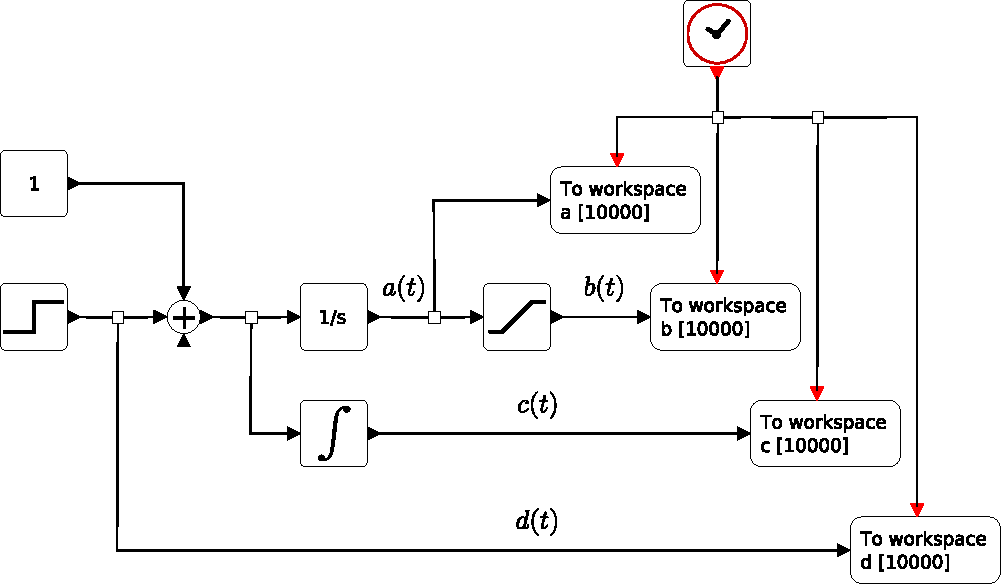
\includegraphics[width=0.8\textwidth]{anti_windup_schemes.pdf} }
	\caption{Схема моделирования, демонстрирующая пару простых реализаций Anti-windup.}
	\label{fig:anti_windup_schemes}
\end{figure}	

\begin{figure}[h!]
	\centering{ 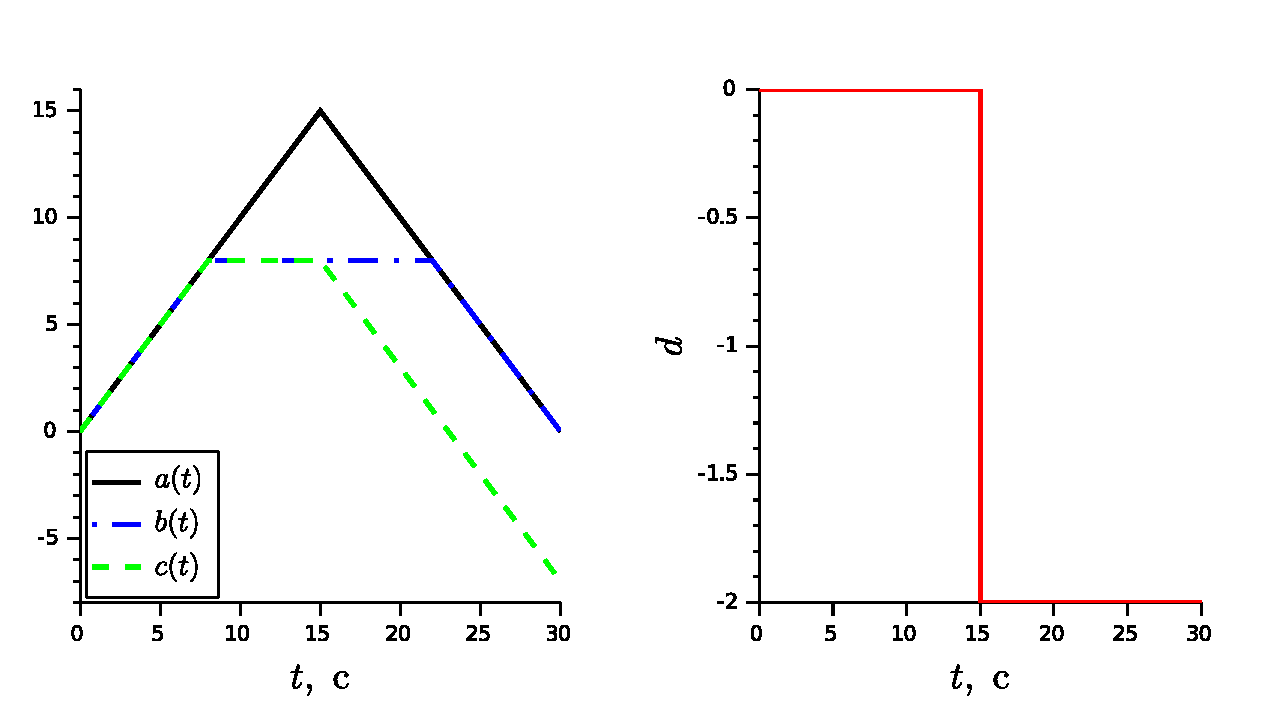
\includegraphics[width=\textwidth]{anti_windup_graphs.pdf} }
	\vspace{-1cm}
	\caption{Графики, поясняющие работу схемы, показанной на рис.~\ref{fig:anti_windup_schemes}.}
	\label{fig:anti_windup_graphs}
\end{figure}	

\begin{figure}[h!]
	\centering{ 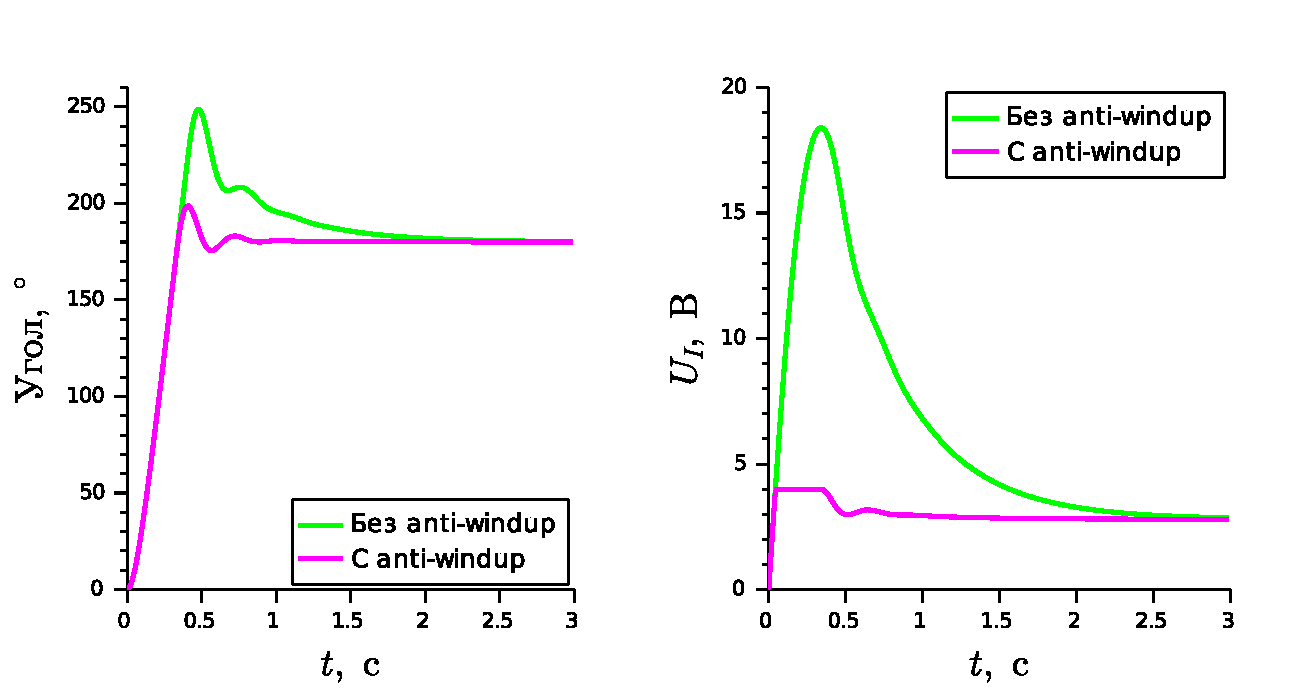
\includegraphics[width=\textwidth]{PI_regul_with_anti_windup.pdf} }
	\vspace{-1cm}
	\caption{Графики, демонстрирующие пользу от применения anti-windup схем.}
	\label{fig:PI_regul_with_anti_windup}
\end{figure}	

ПИД-регулятор, как несложно догадаться, объединяет в себе преимущества всех трех составляющих его регуляторов и, к примеру, для той же схемы моделирования, которая использовалась при рассмотрении ПИ-регулятора, тех же ее параметрах и значении $M_{oth}$ может обеспечить ей переходные процессы, показанные синим и красным цветами на рис.~\ref{fig:PID_graphs_final} (значение $k_D$ для построения этих графиков принималось равным $0.5$).

\begin{figure}[h!]
	\centering{ 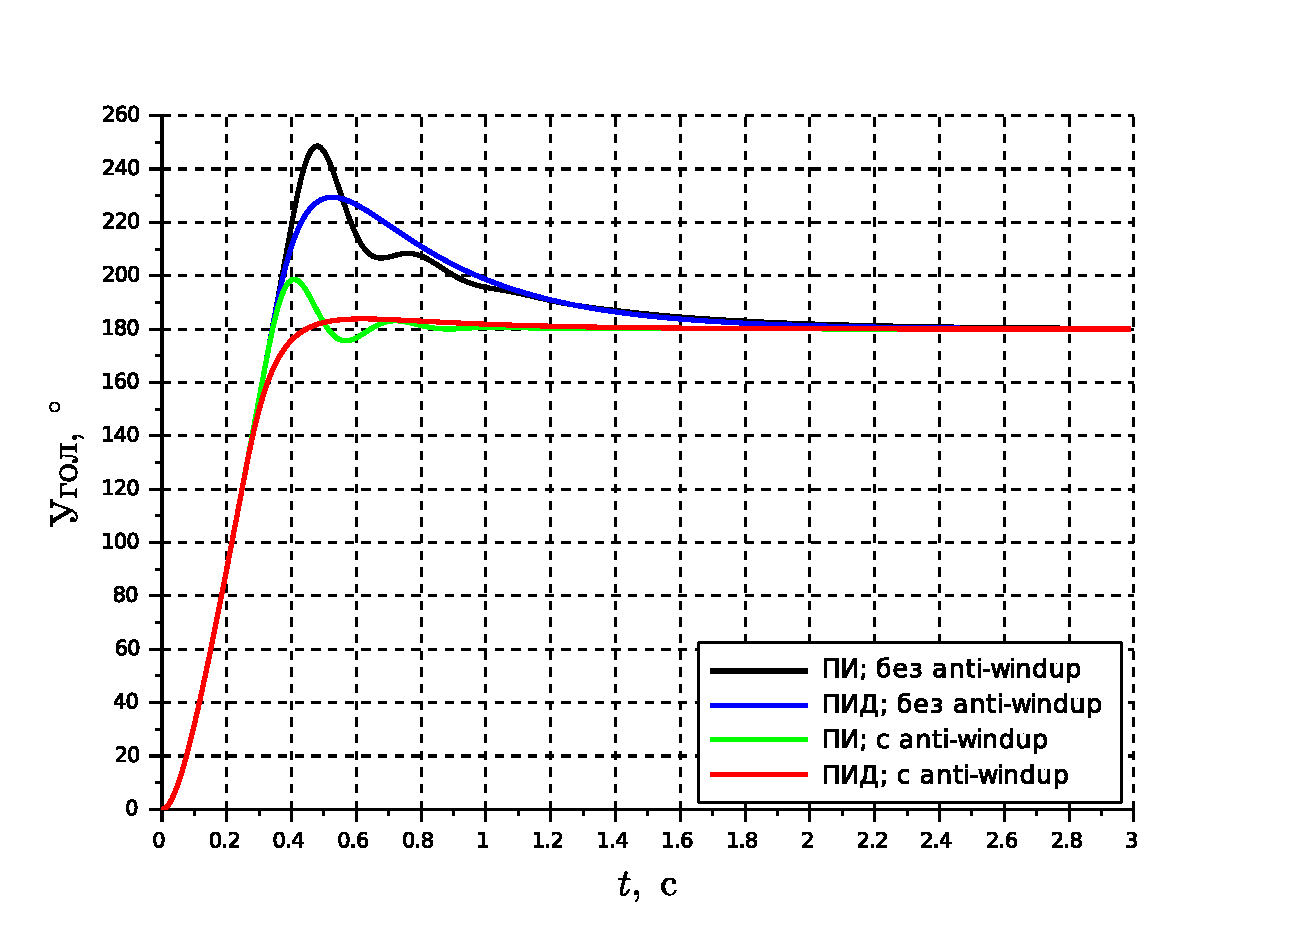
\includegraphics[width=\textwidth]{PID_graphs_final.pdf} }
	\vspace{-1cm}
	\caption{Графики, демонстрирующие возможные кривые для зависимости $\theta(t)$, описывающей работу нагруженного ДПТ, находящегося под управлением ПИ- или ПИД-регулятора.}
	\label{fig:PID_graphs_final}
\end{figure}	

В заключение разговора о ПИД-регуляторе осталось упомянуть о том, откуда берутся значения для его коэффициентов.
Главным образом, можно выделить три источника их возникновения: 1)~ручной, почти ничем не детерминированный или мало детерминированный подбор, 2)~настройка/подбор на основании определенных методик; 3)~обоснованный расчет, опирающийся на какие-нибудь соображения.

\paragraph*{Описание задания работы}$\phantom{-}$\\
\hspace*{\parindent}В~данной лабораторной работе необходимо создать робота-машинку, обладающего дифференциальным приводом\lefteqn,\footnote{Пример такого робота можно видеть в Приложении А.} который, находясь под управлением ПИД-регулятора, мог бы ехать вдоль стены, удерживаясь от нее на определенном расстоянии.
При этом в самом начале своего движения робот не должен быть уже удаленным от стены на необходимое расстояние $d_w=const$.
Таким образом траектория его движения должна быть примерна похожа на ту, которая показана на рис.~\ref{fig:example_of_robots_trajectory}.

\begin{figure}[h!]
	\centering{ 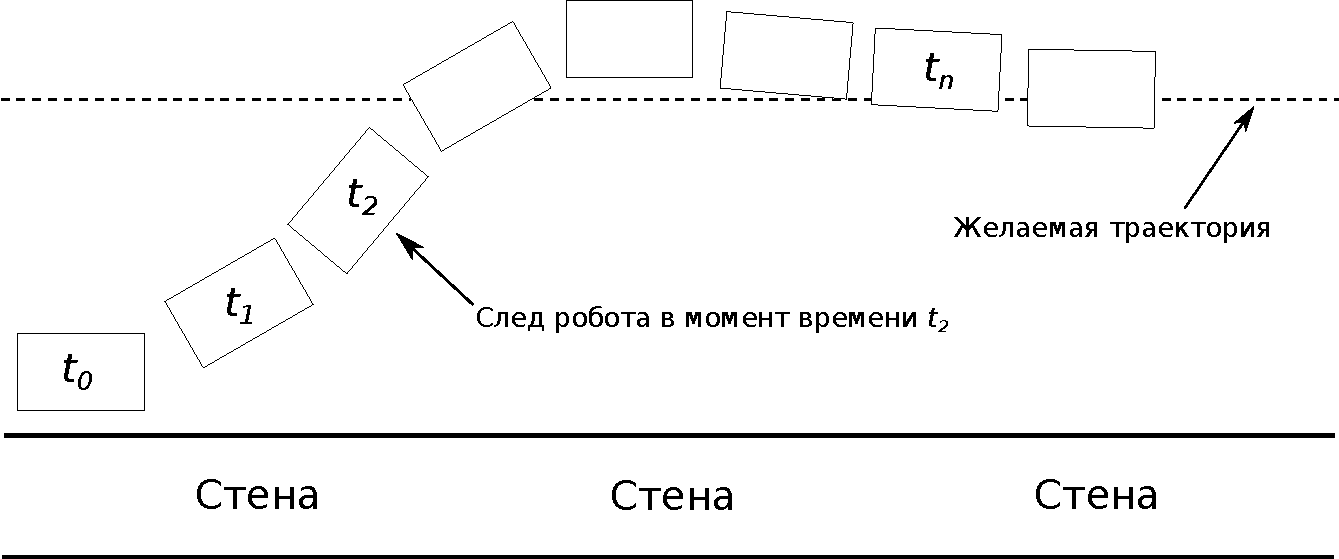
\includegraphics[width=0.8\textwidth]{example_of_robots_trajectory.pdf} }
	\caption{Пример требуемой траектории движения робота.}
	\label{fig:example_of_robots_trajectory}
\end{figure}	

Принцип работы данного робота следующий.
На один из его двигателей подается напряжение, равное $(U_S+U_R)$, на другой~--- $(U_S-U_R)$.
Составляющая полного напряжения $U_S$, б\'oльшая по значению, отвечает за перемещения робота прямо, причем, чем больше значение $U_S$, тем быстрее робот будет перемещаться в указанном направлении.
Вторая составляющая ($U_R$) вызывает поворот робота.
В течение всего времени работы машинки $U_S$ остается постоянным и равным изначально заданному его/ее значению, напряжение же $U_R$ в каждый момент времени подлежит расчету.
Последний в данной работе и предлагается проводить в соответствии с управляющей стратегией ПИД-регулятора на основании отклонения текущего расстояния от робота до стены ($d$) от его желаемого значения $(d_w)$:
\begin{equation}
U_R = k_Pe + k_I\int\limits_{t_0}^{t_1} \!e\,dt + k_D\dot{e},
\end{equation}
где 
\begin{equation}
e = d_w - d\ldotp
\end{equation}

Текущее расстояние робота до стены предлагается определять с помощью двух параллельно направленных дальномеров согласно следующим соображениям.
Угол поворота робота относительно стены ($\alpha$) связан с расстояниями, которые возвращают дальномеры ($d_1$ и $d_2$), выражением (см.~рис.~\ref{fig:distance_finding}):
\begin{equation}\label{eq:tg_alpha}
\tg\alpha = \frac{d_1-d_2}{h},
\end{equation}
где $h$~--- расстояние между дальномерами.
Расстояние правого борта робота до стены ($d$) связано с этими величинами формулой:
\begin{equation}\label{eq:d_in_general}
d = \frac{d_1+d_2}{2}\cdot\cos\alpha\ldotp
\end{equation}
Выражая $\cos\alpha$ через $\tg\alpha$:
\begin{equation}
1+\tg^2\alpha = \frac{1}{\cos^2\alpha} \qquad \Rightarrow \qquad \cos\alpha = \sqrt{\dfrac{1}{1+\tg^2\alpha}},
\end{equation}
подставляя в результат выражение~\eqref{eq:tg_alpha}:
\begin{equation}
\cos\alpha = \sqrt{\displaystyle \dfrac{1}{1 + \dfrac{(d_1 - d_2)^2}{h^2}}}=h\sqrt{\dfrac{1}{h^2+(d_1-d_2)^2}}
\end{equation}
и заменяя тем, что получилось в правой части последнего выражения, $\cos\alpha$ в формуле~\eqref{eq:d_in_general}, для $d$ можно получить следующее:
\begin{equation}
d = 0.5h(d_1+d_2)\sqrt{\dfrac{1}{h^2+(d_1-d_2)^2}}\ldotp
\end{equation}
Собственно, данное выражение и предлагается использовать в программе в качестве расчетной формулы для $d$.

\begin{figure}[h!]
	\centering{ 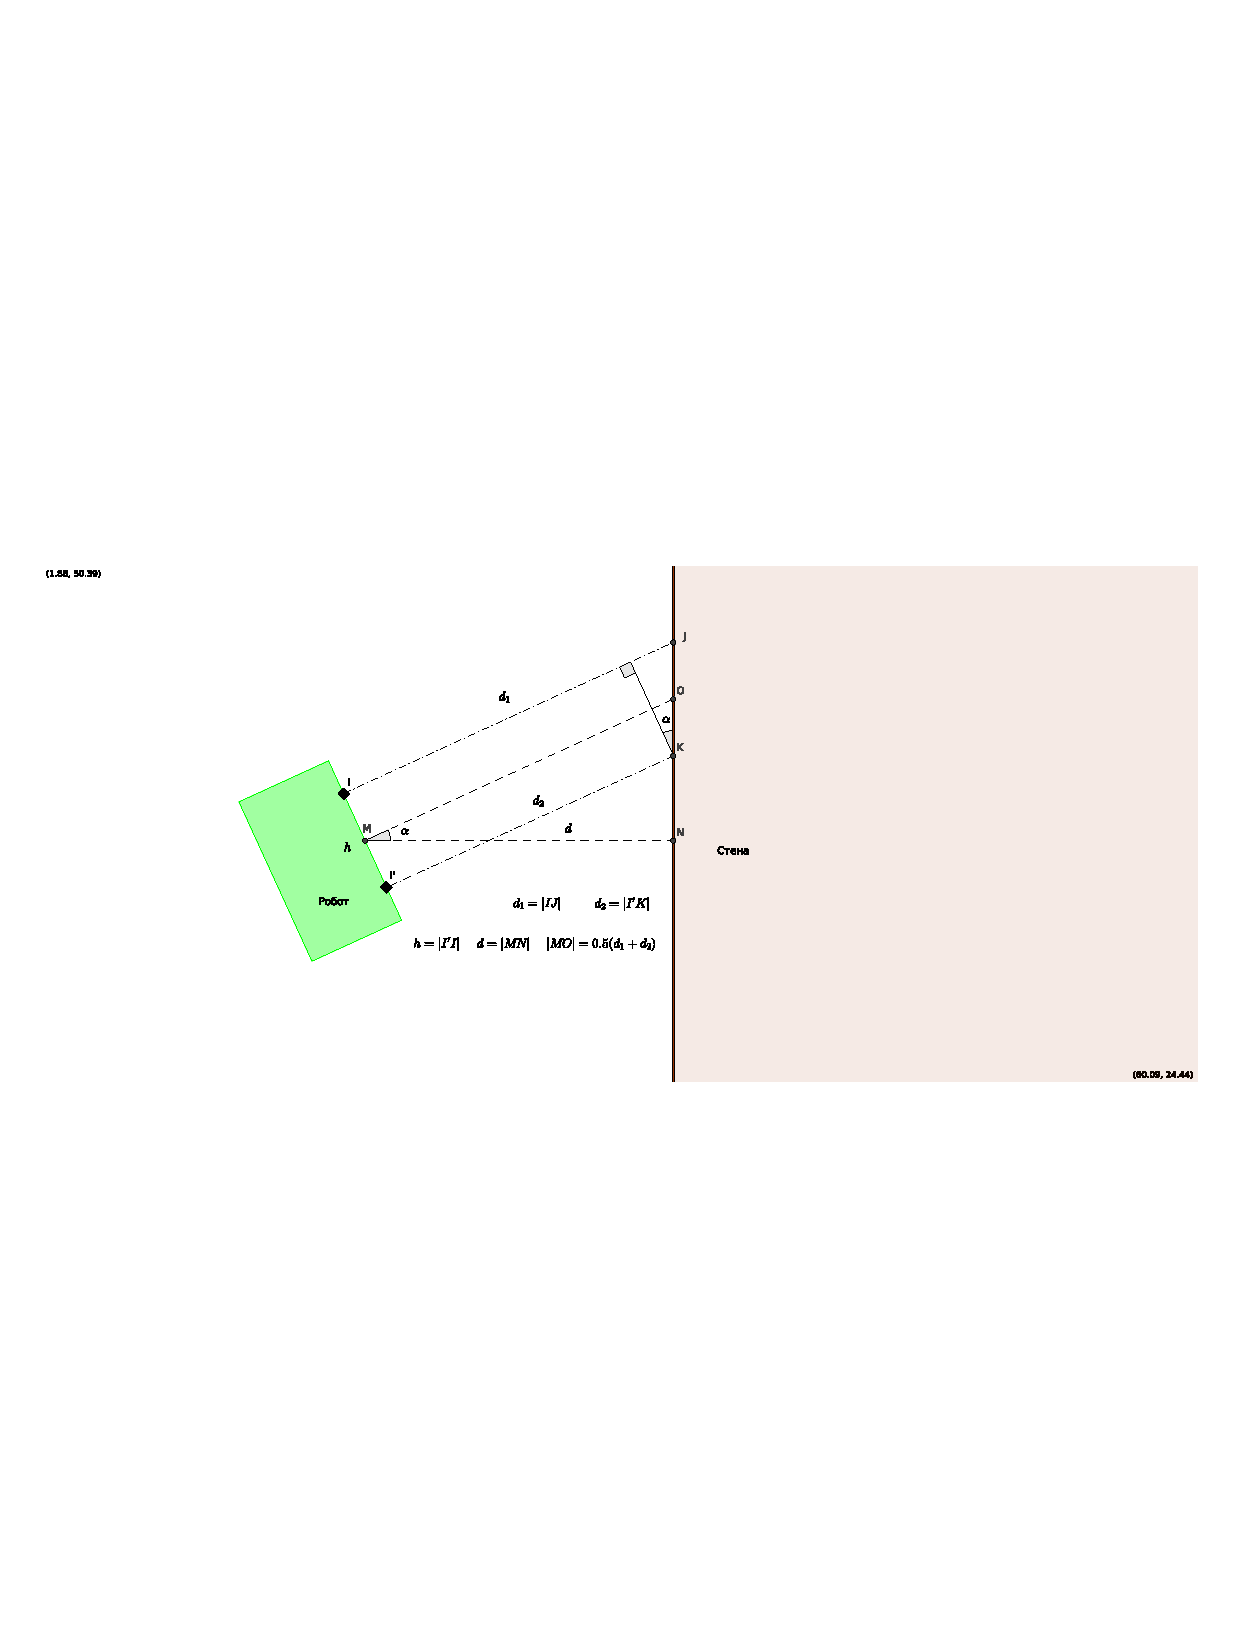
\includegraphics[width=0.9\textwidth]{j.pdf} }
	\caption{Пояснение к поиску расчетной формулы для $d$.}
	\label{fig:distance_finding}
\end{figure}
\newpage
{$\phantom{-}$}
\newpage				 
\section{Цель работы}
\hspace*{\parindent}Познакомиться с концепцией ПИД-регулятора.
Получить опыт настройки его параметров, решив определенную задачу управления для мобильного робота с дифференциальным приводом.

\section{Порядок выполнения работы}
\begin{enumerate}
\item Соберите робота-машинку, на основе которого возможно проделать необходимые эксперименты.
Конструкция одного из таких роботов представлена в приложении~А.
\item \label{item:program_task}Напишите для него программу, которая, используя ПИД-регулятор, организует описанное в подразделе <<Описание задания работы>> основной части методического пособия поведение робота.
\item Следуя указанной преподавателем методике подбора параметров ПИД-регулятора, определите значение его коэффициентов $k_P$, $k_I$ и $k_D$ и параметры anti-windup схемы, при которых поведение робота будет удовлетворять оговоренным преподавателем требованиям.
\item На основании данных, полученных с помощью программы из п.~\ref{item:program_task} в течение процесса настройки ПИД-регулятора, постройте с помощью Scilab указанные преподавателем графики для зависимости $d(t)$.
\end{enumerate}

\section{Содержание отчета}
\begin{enumerate}
\item Все графики, предусмотренные разделом <<Порядок выполнения работы>>, с указанными значениями коэффициентов ПИД-регулятора и параметрами anti-windup схем.
\item Исходный код управляющей роботом программы.
\item Выводы о результатах проделанной работы.
\end{enumerate}

\newpage
\section*{Приложение А\\
Пример подходящего для экспериментов робота-машинки.}
\hspace*{\parindent}Конструкцию одного из роботов, с использованием которого возможно проделать необходимые эксперименты, описывают рис.~\ref{fig:first_append_fig}--\ref{fig:last_append_fig}.
\vspace{1cm}
\begin{figure}[h!]
	\centering{ 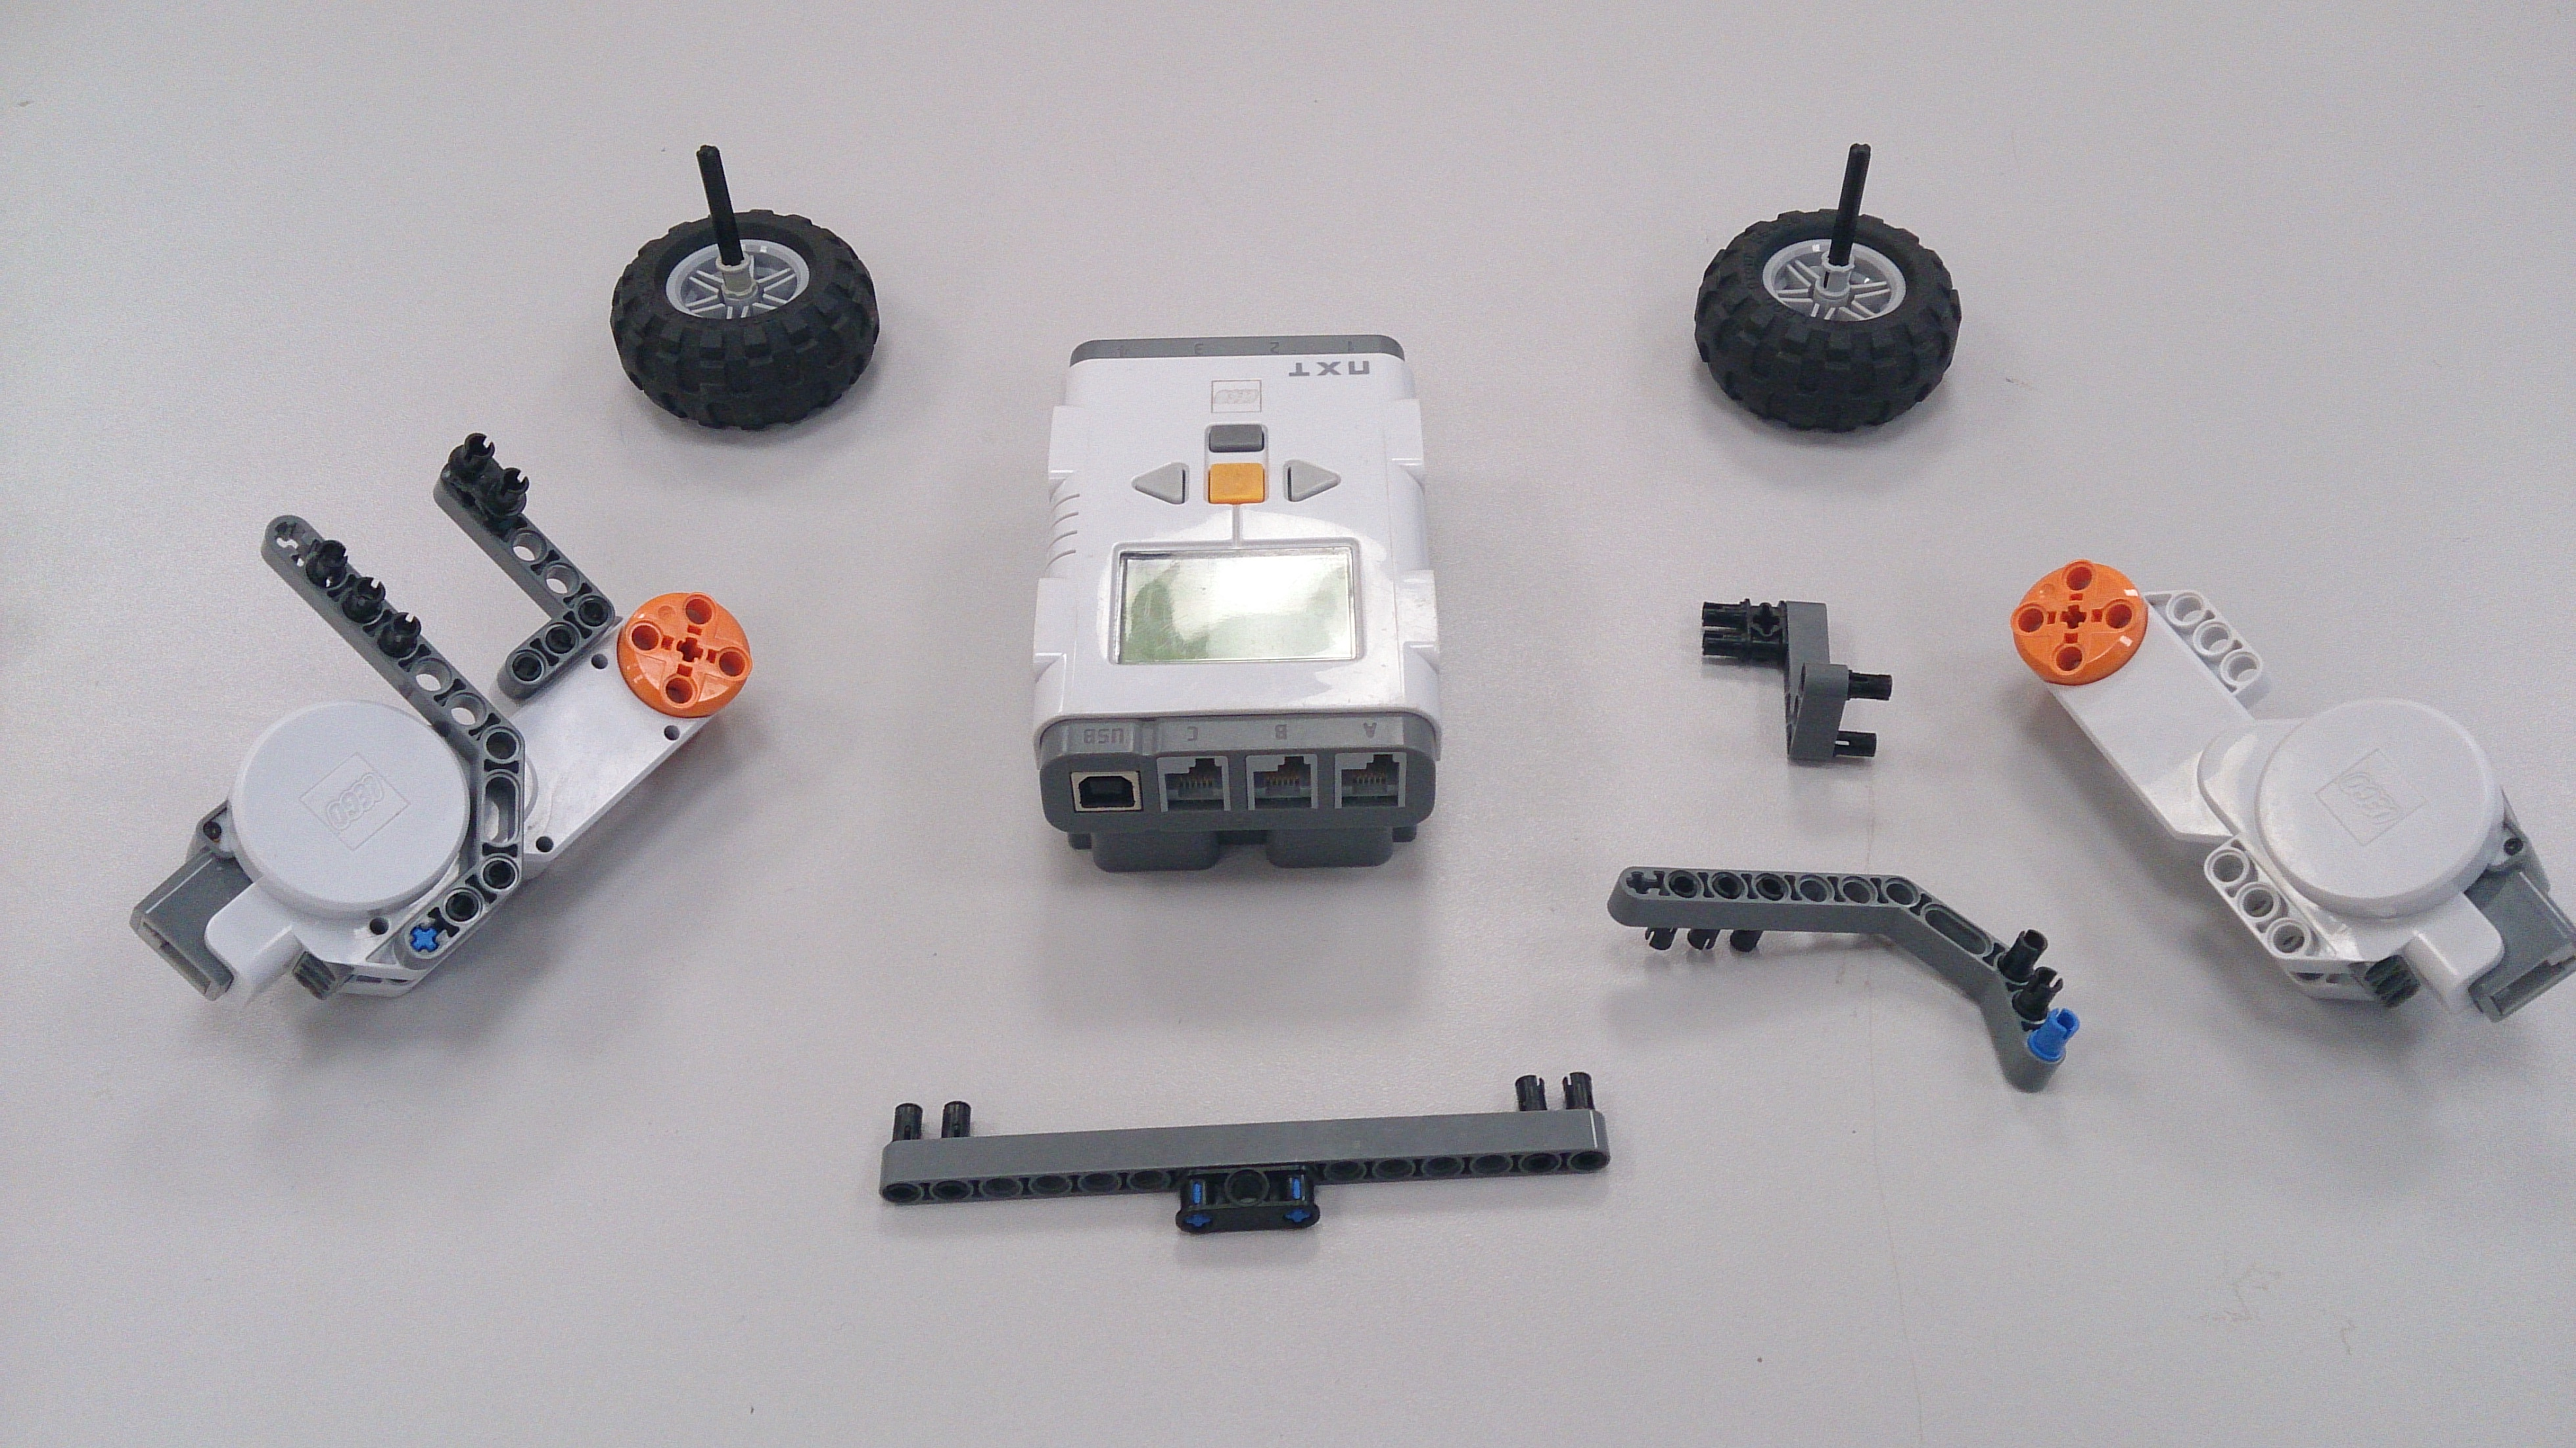
\includegraphics[width=\textwidth]{main_parts.JPG} }
	\vspace{-0.5cm}
	\caption{Основные детали робота.}
	\label{fig:first_append_fig}
\end{figure}	
\vspace{1cm}
\begin{figure}[h!]
	\centering{ 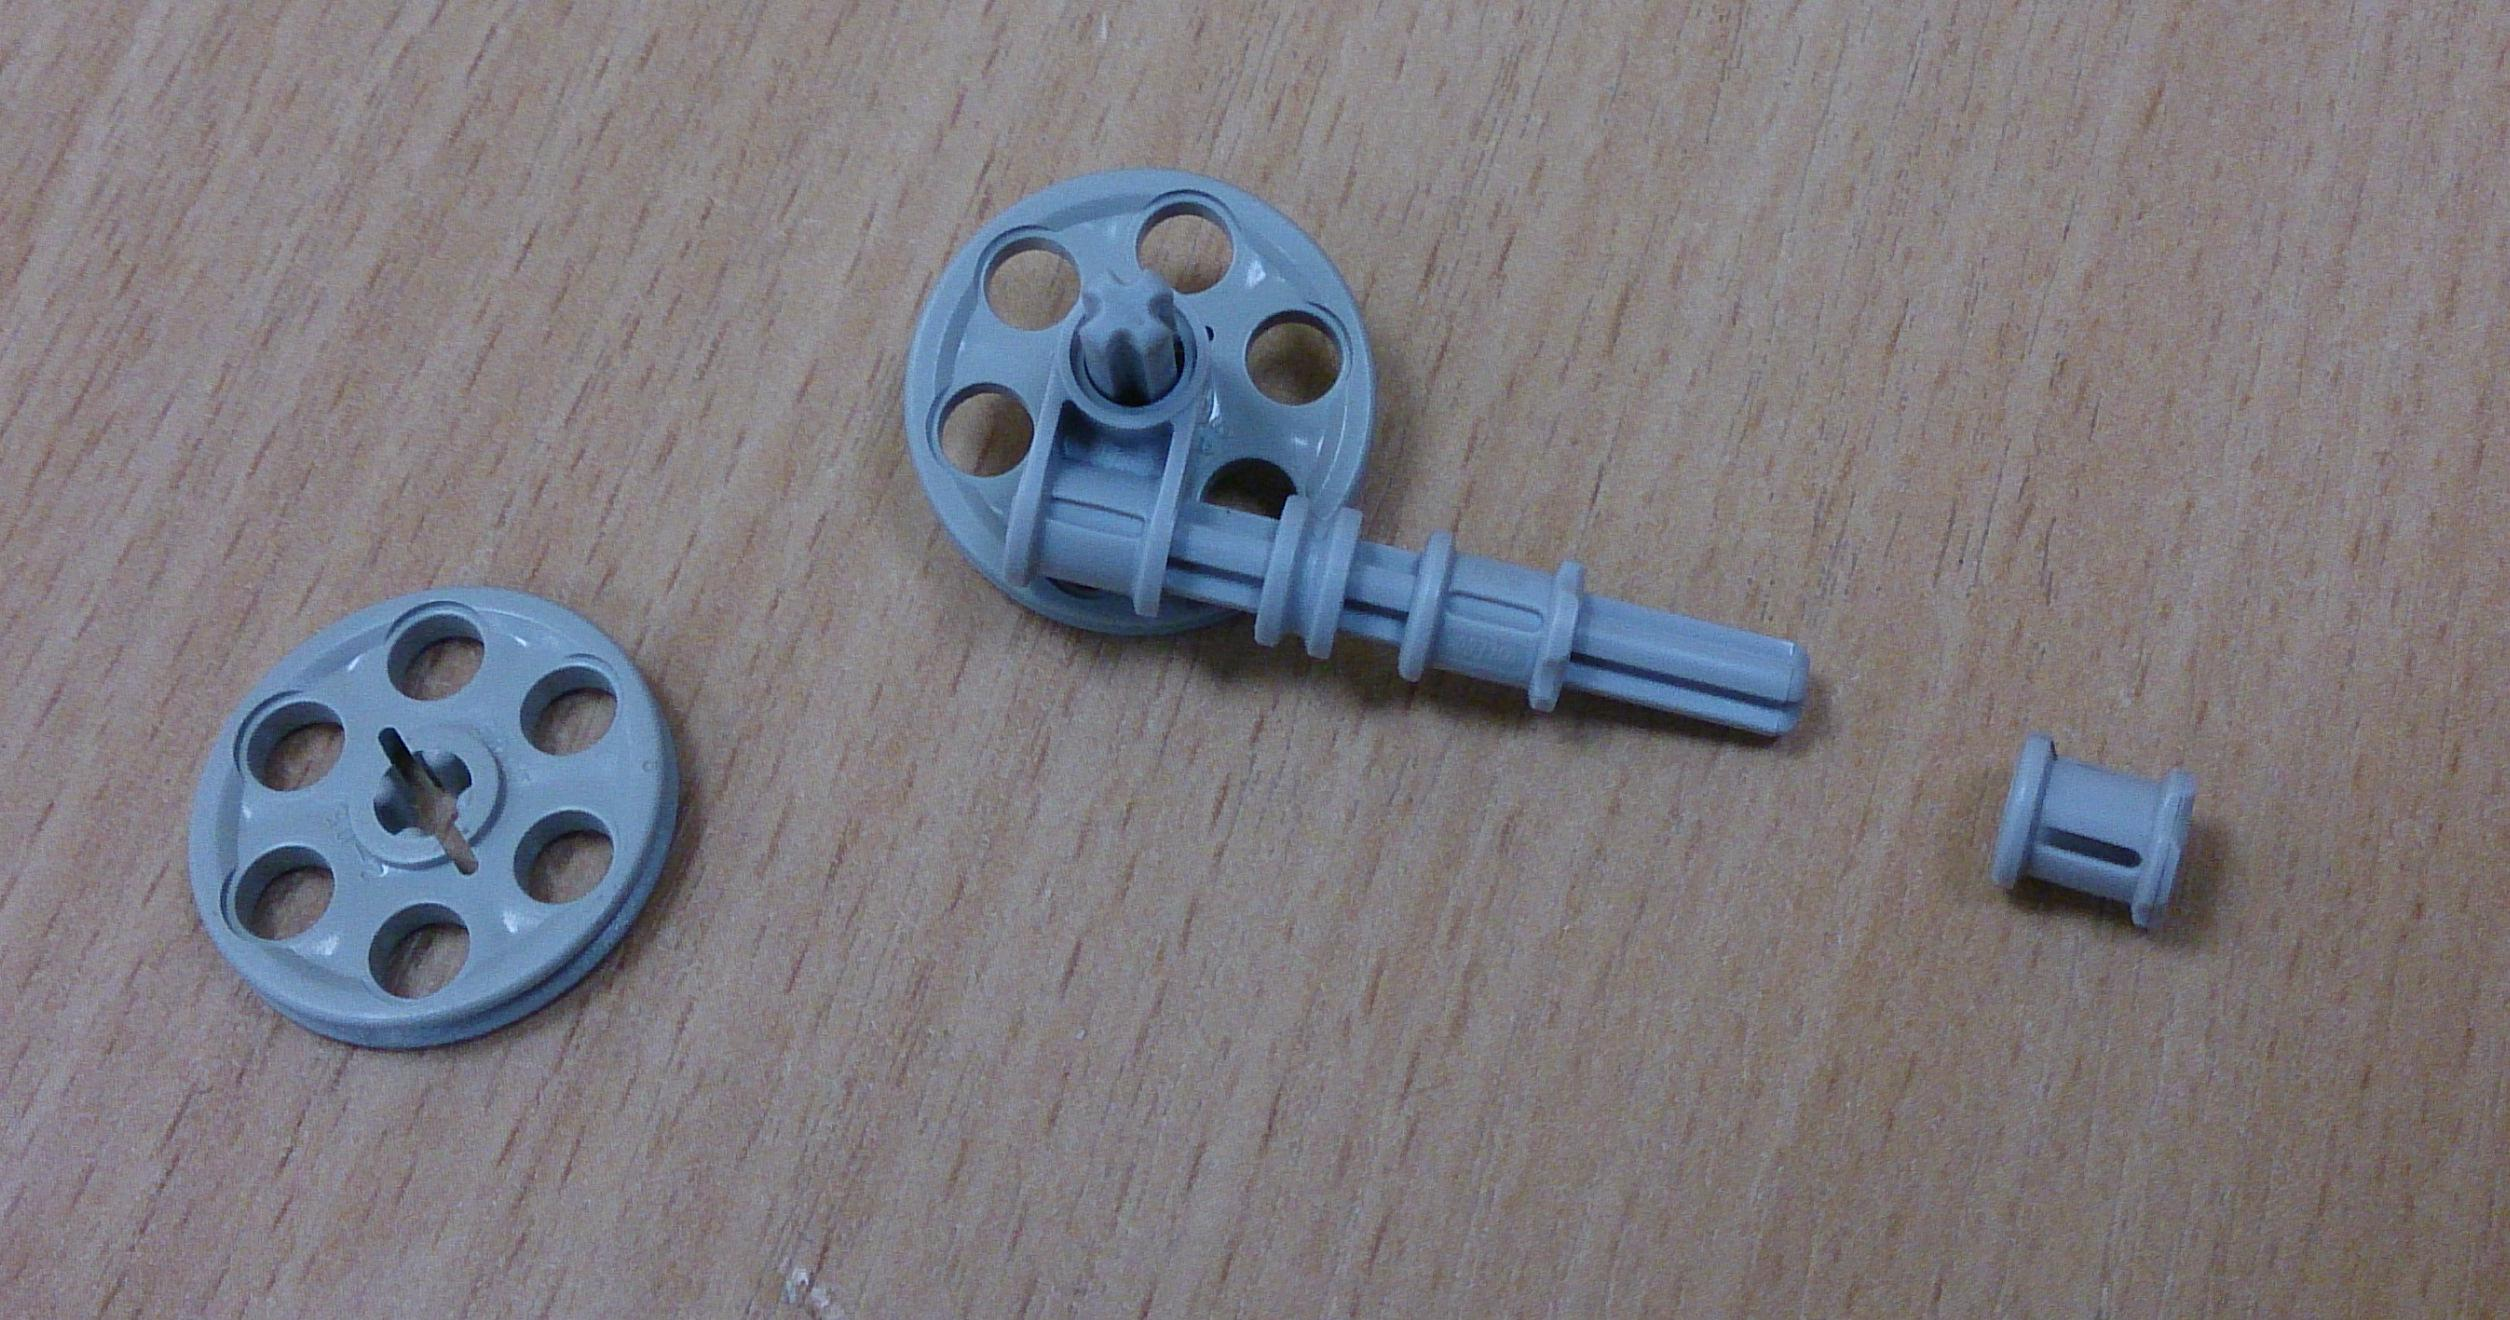
\includegraphics[scale=0.12]{front_wheel.jpg} }
	\caption{Строение переднего колеса.}
\end{figure}	
	
\begin{figure}[h!]
	\centering{ 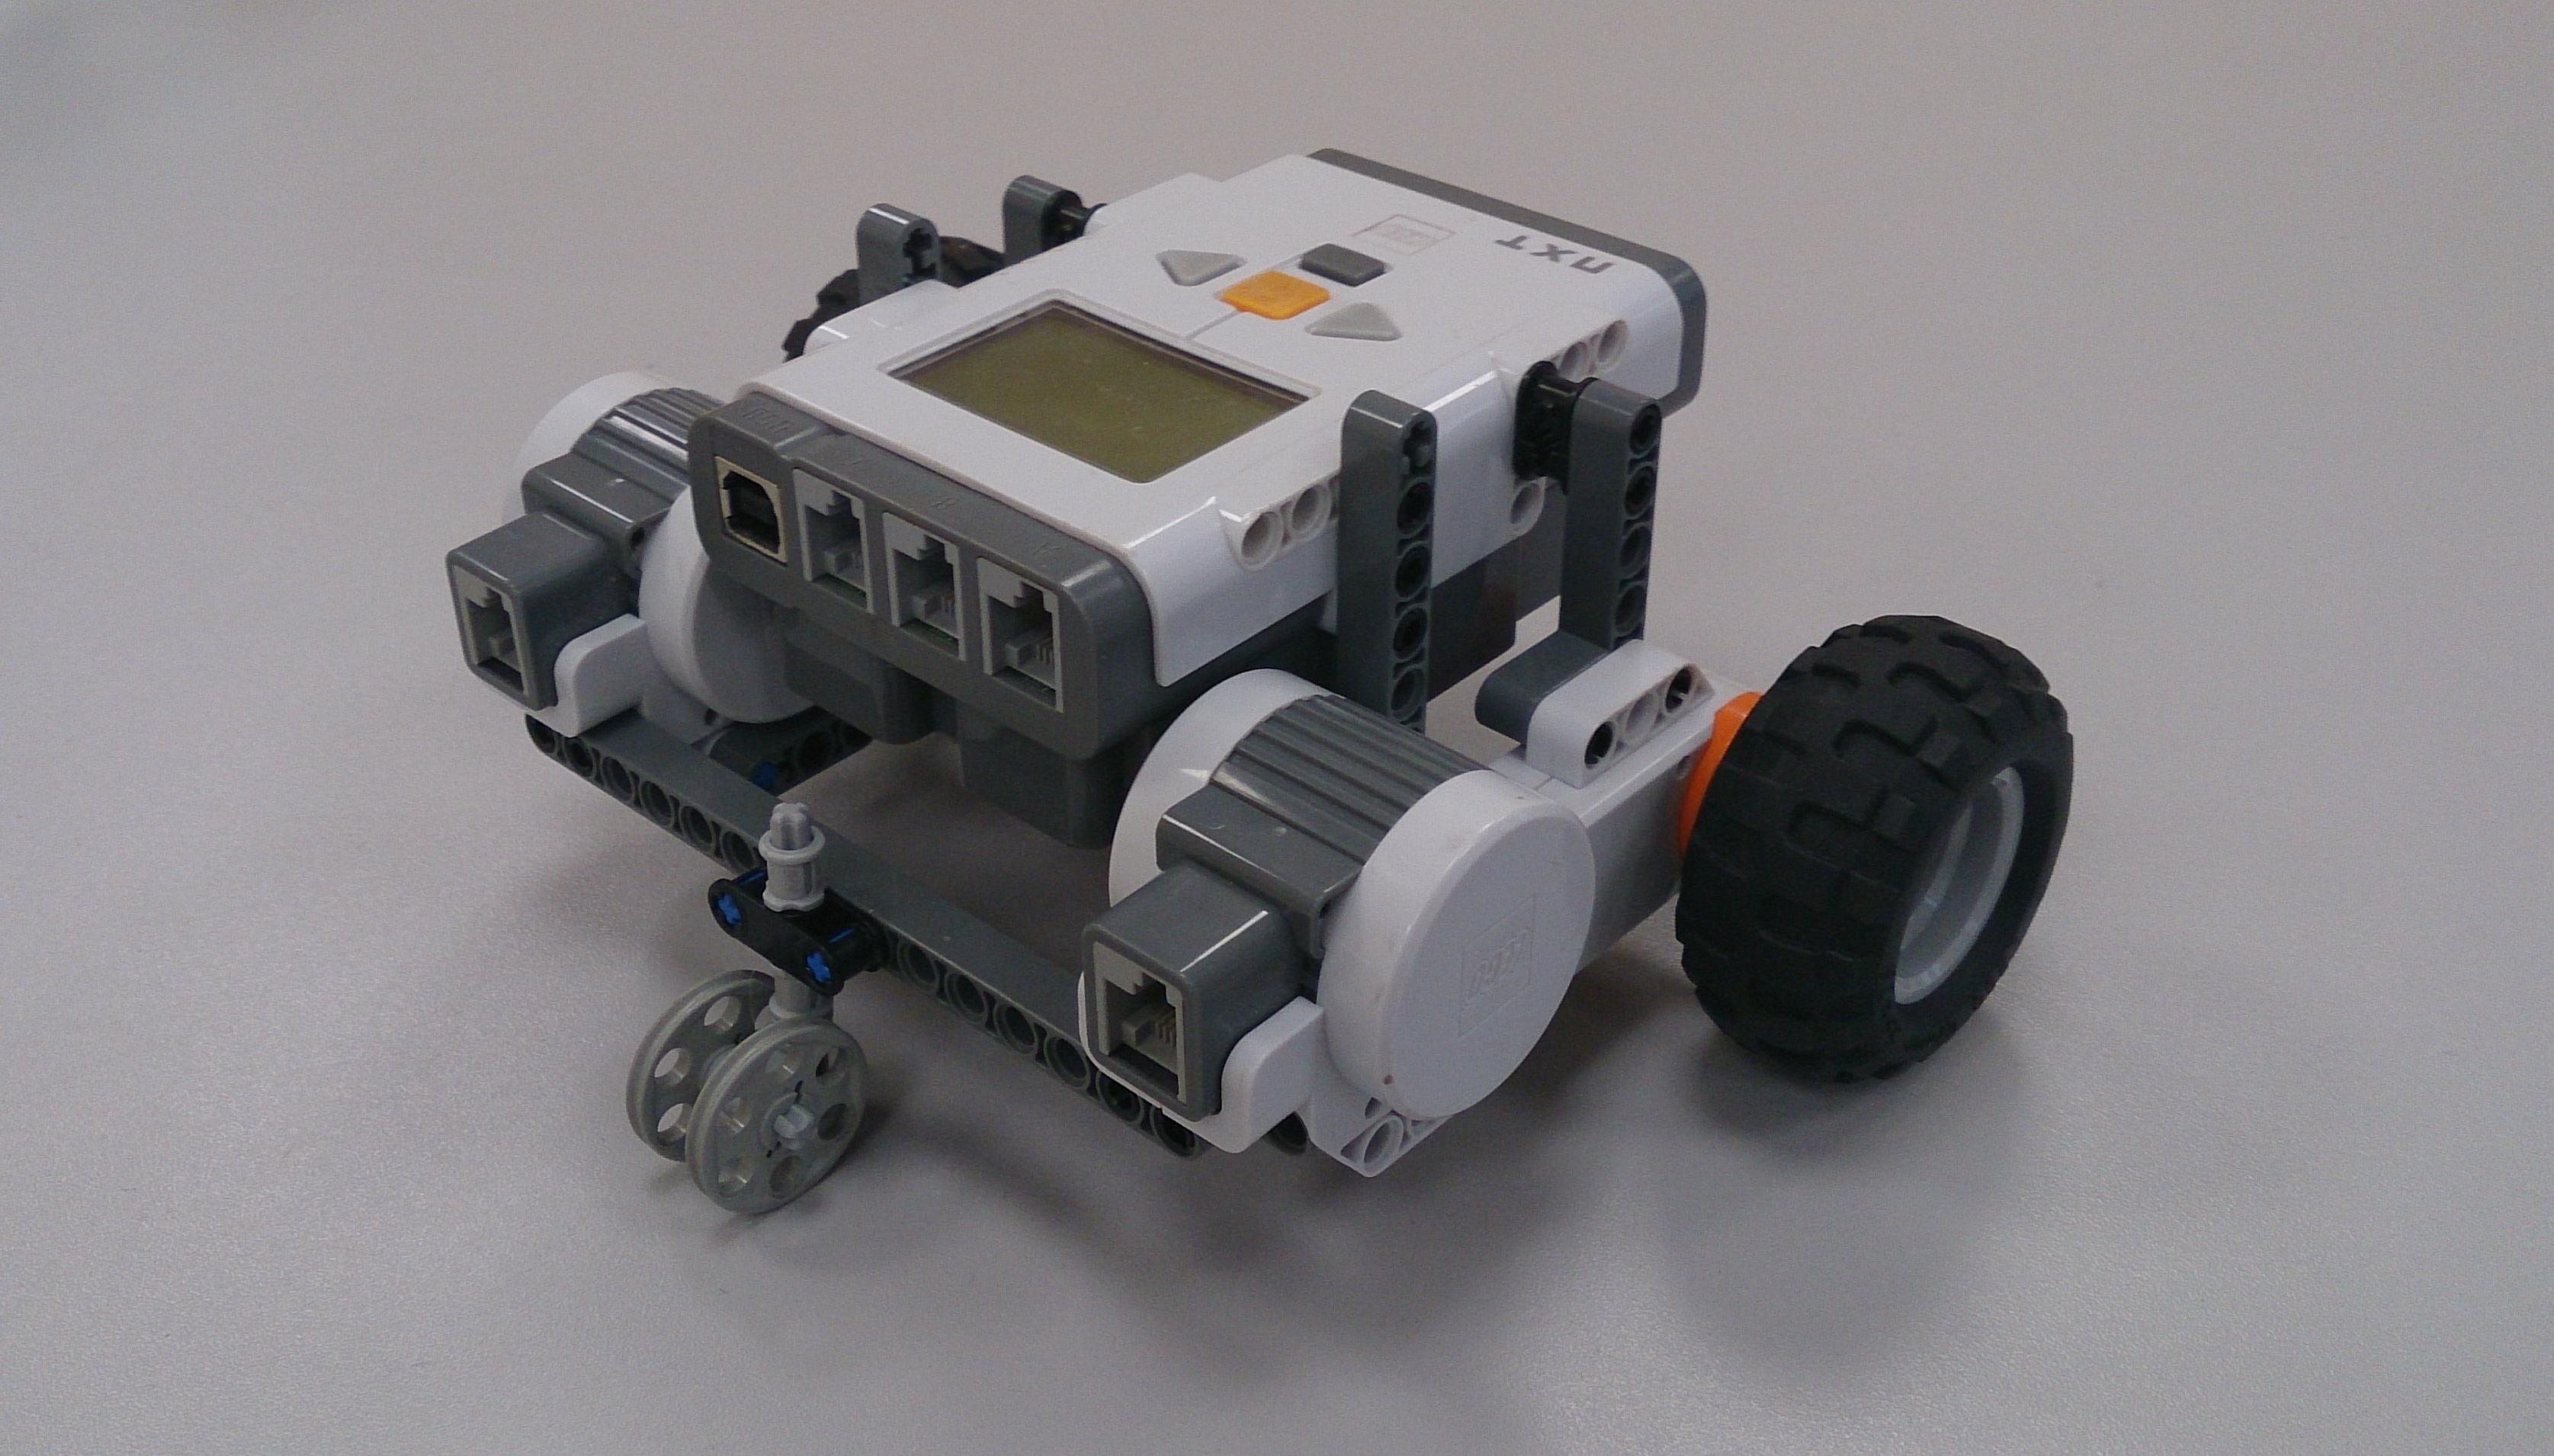
\includegraphics[width=\textwidth]{move_part.jpg} }
	\caption{Основная часть робота в собранном виде.}
\end{figure}		

\begin{figure}[h!]
	\centering{ 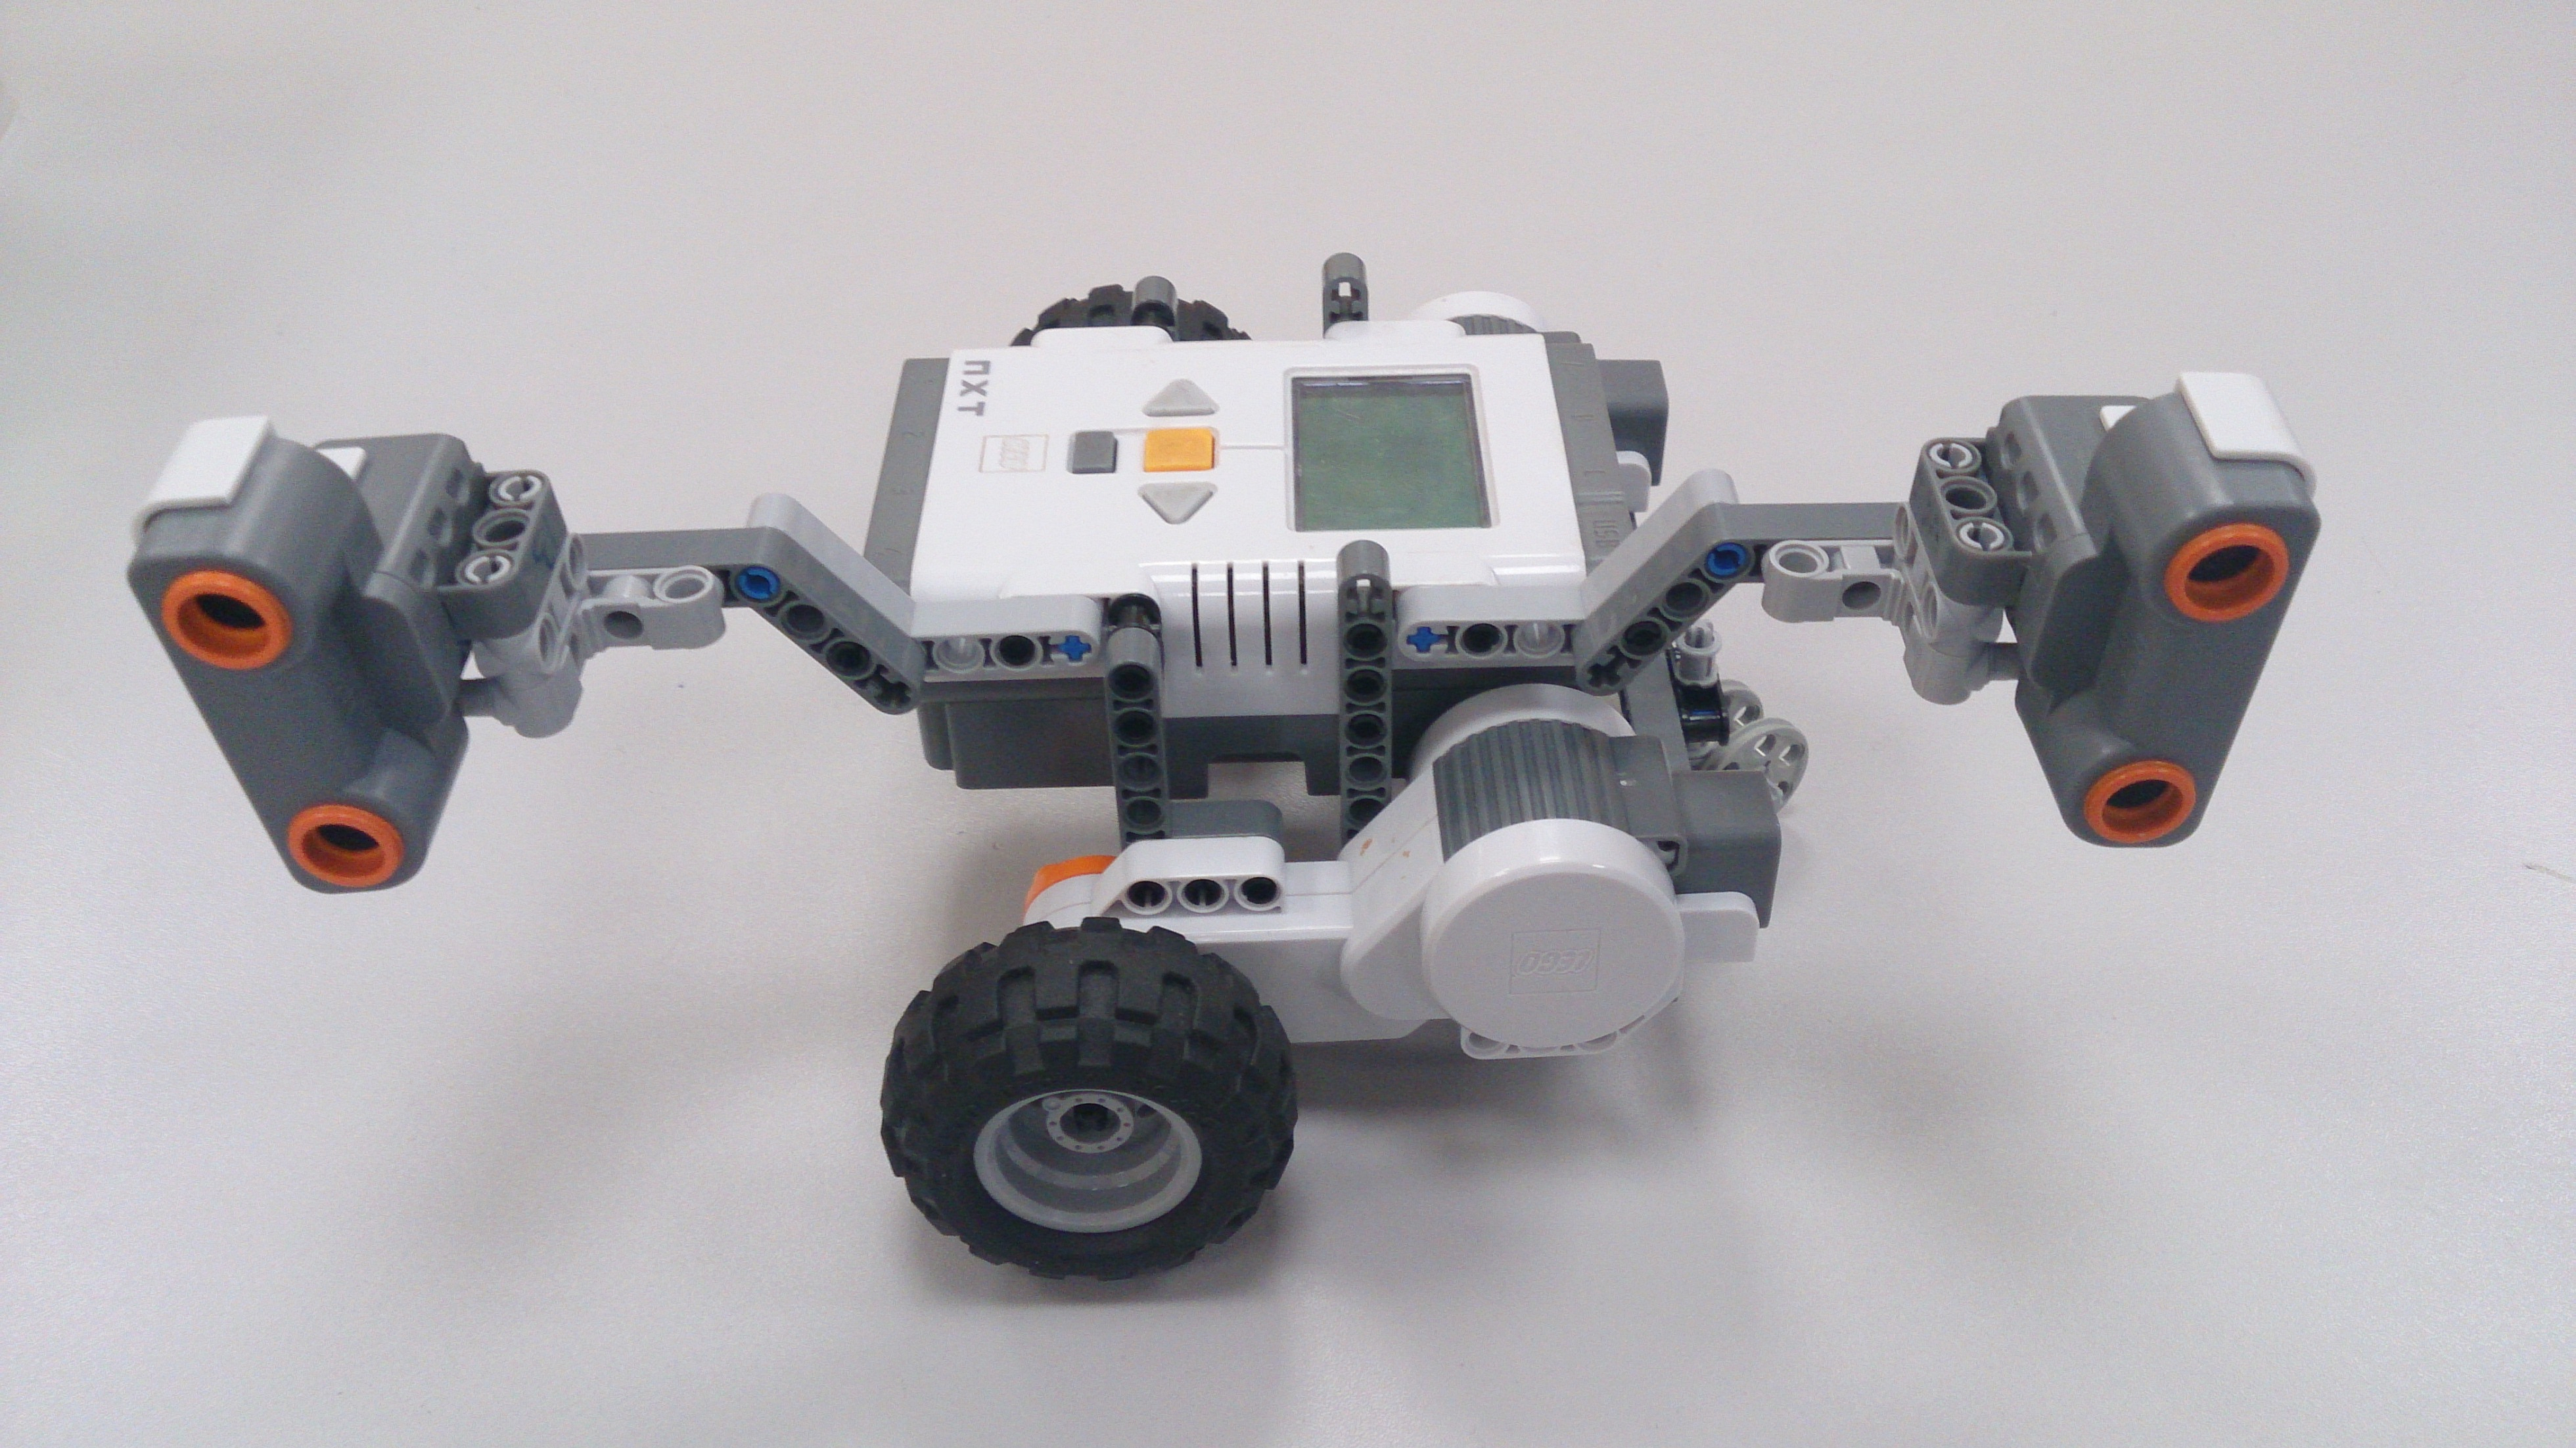
\includegraphics[width=\textwidth]{full_robot.JPG} }
	\caption{Полностью собранный робот.}
	\label{fig:last_append_fig}
\end{figure}	
	
\end{document}
